\chapter{Progettazione del sistema SCADA}

La progettazione di un sistema SCADA è un processo articolato e strategico, che richiede attenta pianificazione e un ampio impiego di risorse. Senza una struttura ben definita, infatti, si possono generare configurazioni di prodotto che necessitano di essere successivamente ripensate, portando inevitabilmente a un incremento di costi, non solo in termini di tempo, ma anche di risorse umane.
Per garantire un corretto avanzamento e rispondere in modo efficiente alle aspettative del cliente, è buona norma suddividere il lavoro in fasi predeterminate. In tal modo, si può procedere con maggiore chiarezza, sapendo già dal principio quali aspetti richiederanno attenzione specifica nelle varie fasi del progetto. Nel mio caso, il lavoro è stato suddiviso in quattro fasi principali:
\begin{enumerate}
    \item Analisi dei requisiti
    \item Strutturazione dell'HMI
    \item Gestione Database
    \item Sviluppo back-end con integrazione al PLC
\end{enumerate}
Ognuna di queste fasi ha contribuito in modo sostanziale a preservare la coerenza e l'integrità del prodotto finito, consentendo di ottenere un risultato che rispecchiasse fedelmente le richieste.

\section{Analisi dei requisiti del cliente}

La prima fase - definita anche come fase di design - prevede un momento di dialogo approfondito con il cliente per comprendere e prendere nota di tutte le necessità, in modo da tradurle in specifiche dettagliate, misurabili e quindi concretamente realizzabili dal team. L'analisi dei requisiti prevede diverse attività, la cui applicazione varia in base alla natura del prodotto finale. Oltre alla raccolta, è fondamentale l'organizzazione del loro sviluppo, soprattutto nei progetti più complessi in cui è necessario stratificare il lavoro tra più individui. 

Per quanto riguarda il mio progetto, dato l'obiettivo di creare un sistema che potesse essere altamente modulare e in grado di costituire una base solida per futuri progetti, mi è stato richiesto di soffermarmi su alcuni aspetti di fondamentale rilevanza:
\begin{enumerate}
    \item Creare un'interfaccia quanto più user-friendly possibile, per facilitare l'utilizzo e l'accessibilità da parte degli operatori di macchina.
    \item Definire un "ricettario" di base, ovvero una struttura configurabile e facilmente aggiornabile, sotto il nome di "anagrafica articoli".
    \item Definire una sezione dedicata agli ordini di produzione che includa sia i comandi di produzione per la gestione operativa, sia gli storici. 
    \item Implementare un sistema efficiente per la gestione e l'accesso agli allarmi e warning, essenziale per il monitoraggio e la diagnostica.
    \item Creare scorciatoie che permettono allo sviluppatore di poter testare il prodotto sia in fase di sviluppo, che a prodotto finito, anche tramite tele-assistenza.
\end{enumerate}

\section{Strutturazione HMI (Human Machine Interface)}
Per la realizzazione dell'HMI, l'azienda mi ha mostrato altri prodotti fornendomi le basi per comprendere il funzionamento delle interfacce. Dopo aver ricevuto piena autonomia decisionale da parte dell'azienda, ho sviluppato un approccio originale, scegliendo di procedere nel seguente modo. All'interno di FT Optix™, per prima cosa l'interfaccia è stata organizzata in una finestra principale denominata \textit{MainWindow}\textsuperscript{\cite{rockwelloptixmainwindow}} (Figura \ref{fig:HMI00.png}), a sua volta suddivisa in 3 sotto-pannelli:
\begin{itemize}
    \item Pannello di stato
    \item Pannello di funzione
    \item Pannello di menù
\end{itemize}
Il \textbf{Pannello di stato} è un elemento presente in tutta l'interfaccia e di conseguenza visibile in ogni menù e sotto-menù. La sua presenza è fondamentale poiché contiene al suo interno informazioni per il funzionamento dell'interfaccia stessa. Procedendo da sinistra troviamo il logo dell'azienda produttrice dell'impianto, che in questo caso è Rea Robotics, per dare riconoscibilità e identità a tutto il sistema. Subito dopo è presente un indicatore che contiene il nome dell'operatore che sta utilizzando la macchina (di default impostato ad anonimo). Se viene selezionato, apre un menù a tendina da cui è possibile poter eseguire l'accesso, sia come operatore, sia come sviluppatore. Tale distinzione è importante perché alcune funzioni dell'interfaccia sono accessibili solo a figure autorizzate come gli sviluppatori, per garantire sicurezza e integrità delle operazioni. 
Continuando verso destra è presente l'orario, utile per avere sempre sotto controllo il tempo durante le operazioni, e il pulsante per la selezione della lingua, che mostra l'icona della lingua attualmente attiva: l'interfaccia è stata progettata per poter funzionare sia in lingua italiana sia in lingua inglese, garantendo maggiore adattabilità anche in ambienti internazionali. Infine è presente il pulsante di spegnimento, che permette di chiudere l'interfaccia in modo sicuro. Per prevenire chiusure accidentali, alla pressione appare un popup che richiede un'ulteriore conferma di spegnimento della macchina, evitando che un tocco involontario possa interrompere il lavoro dell'operatore.
Nella parte inferiore di questo pannello è presente una sezione blu che si occupa di monitorare lo stato degli allarmi e avvisi. In caso di problemi, tale sezione mostra chiaramente l'allarme e la descrizione rilevata, assicurando così pronta visibilità delle condizioni operative del sistema.

\begin{figure} 
    \centering
    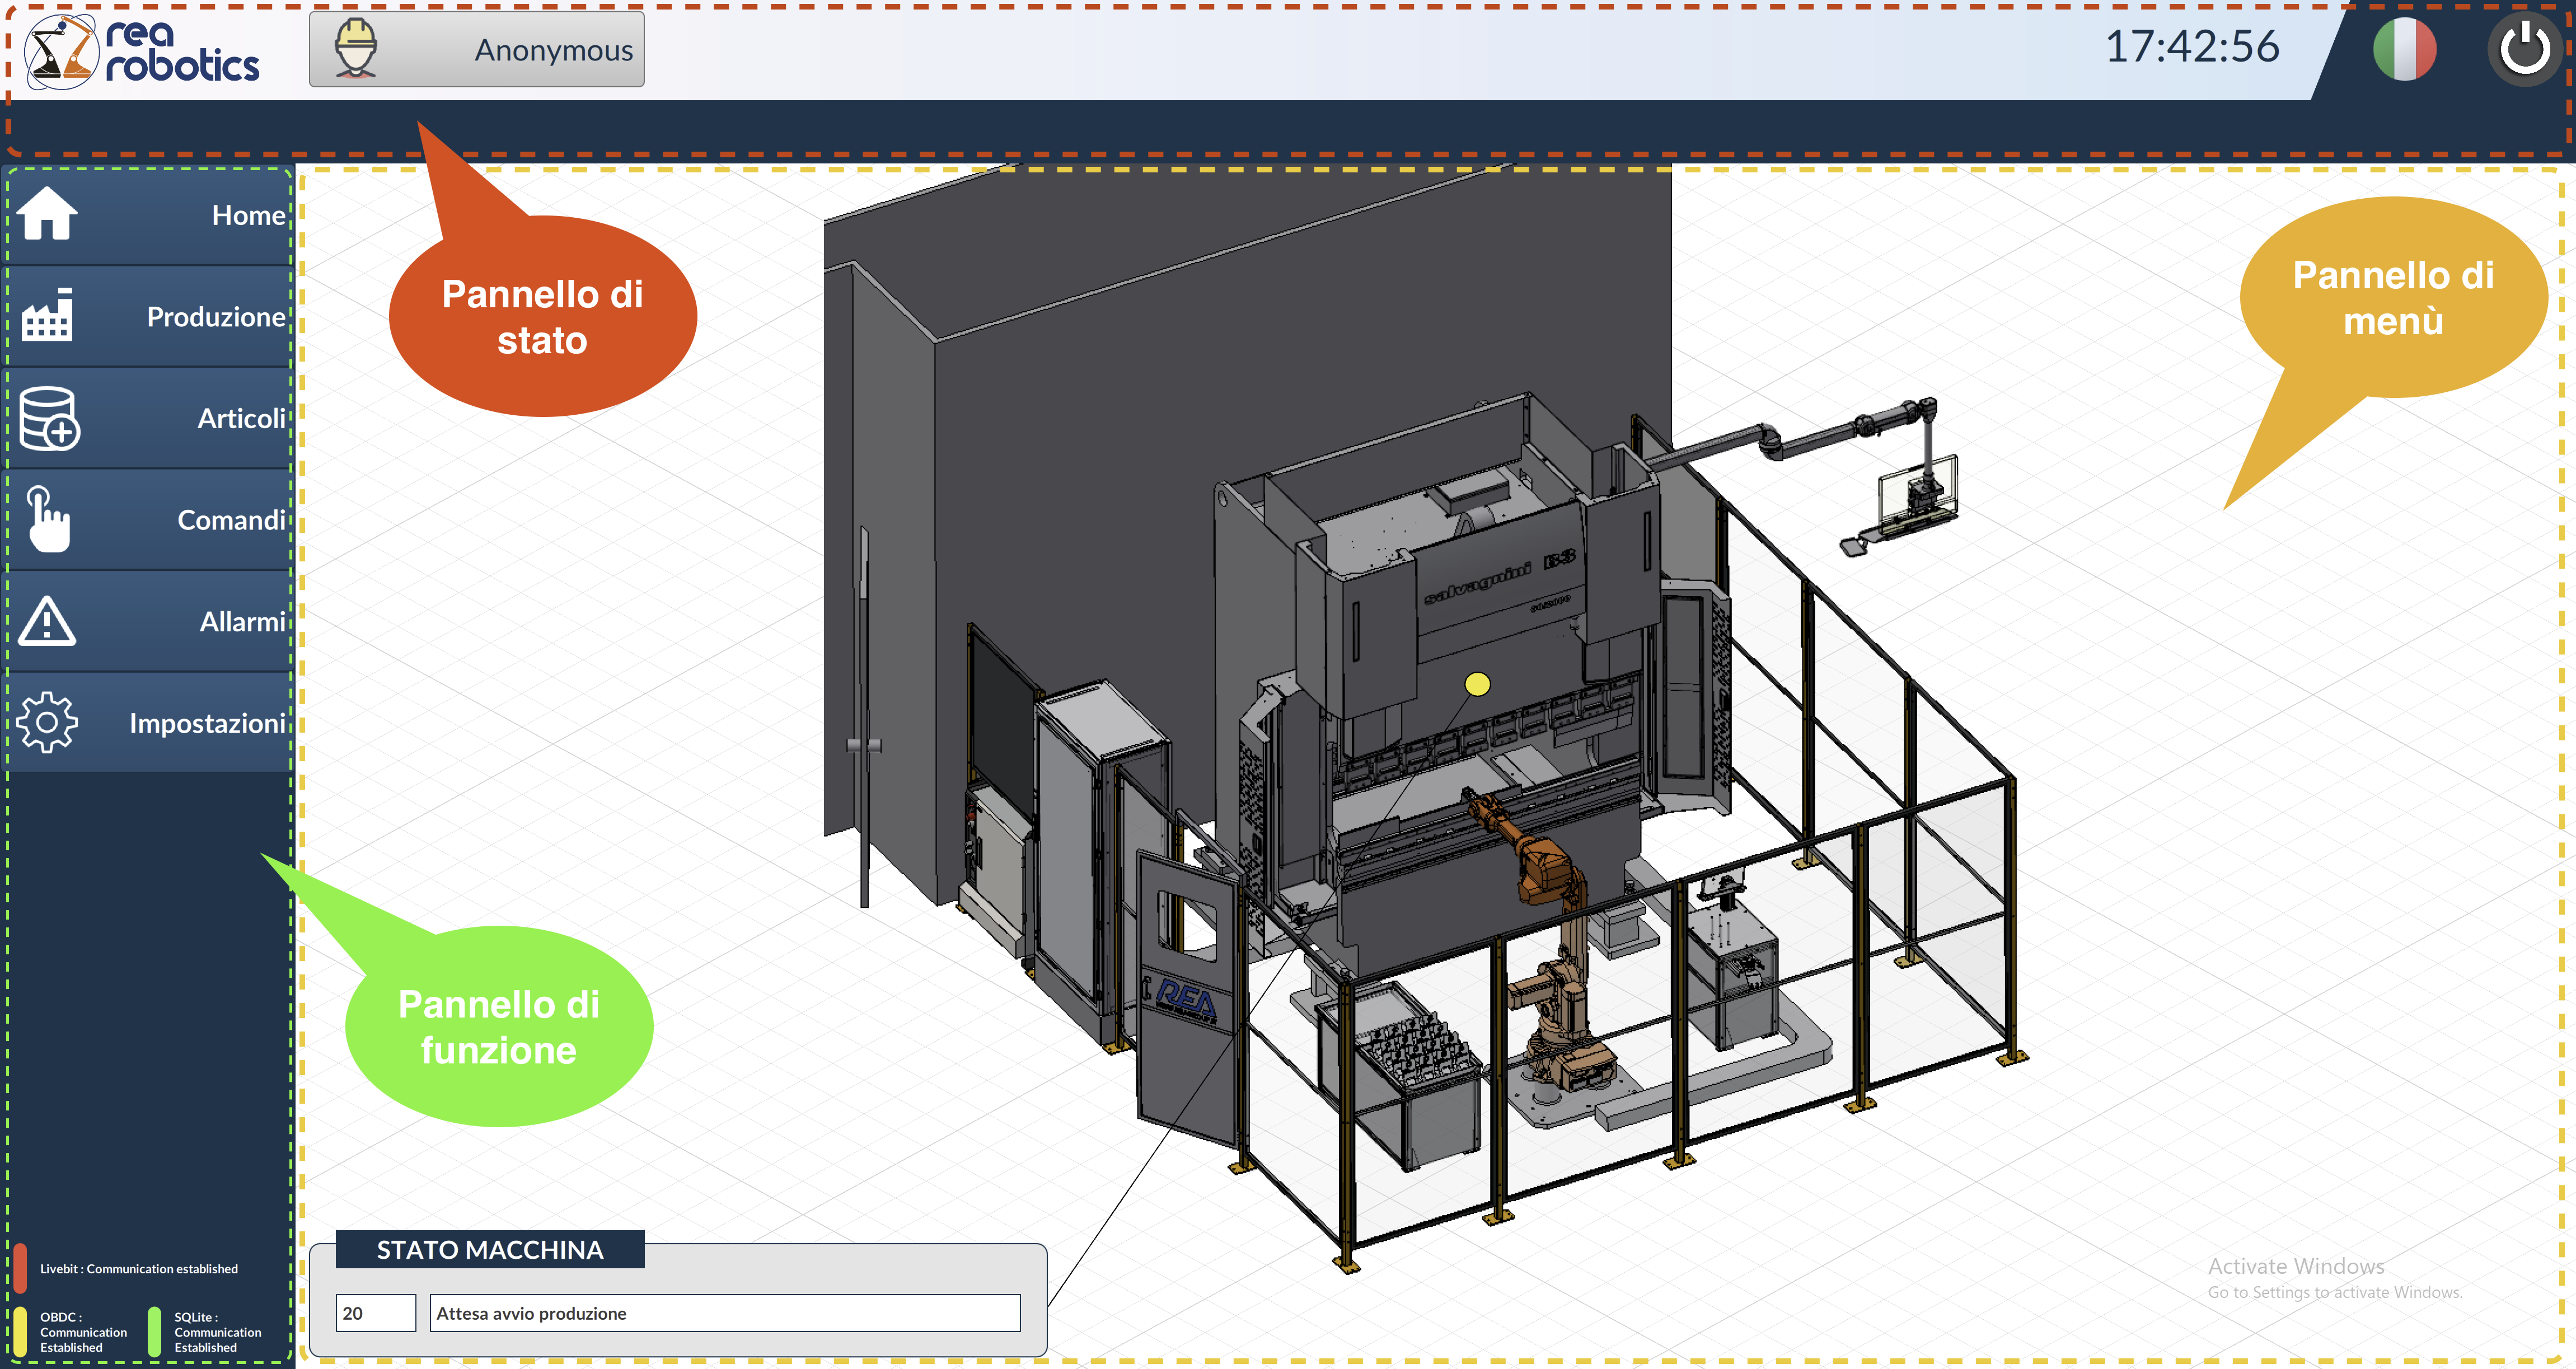
\includegraphics[width=1\linewidth]{Immagini/HMI00.png}
    \caption{Suddivisione interfaccia HMI}
    \label{fig:HMI00.png}
\end{figure}

Il \textbf{Pannello di funzione}, come il pannello di stato, è un elemento fisso che permette la navigazione attraverso i vari menù. Questo pannello è costituito da un layout verticale con una serie di pulsanti che consentono all'operatore di accedere a tutte le principali sezioni dell'interfaccia. Ogni pulsante identifica un menù specifico e, una volta selezionato, consente di passare rapidamente alla schermata desiderata, interagendo dinamicamente con il pannello di menù posizionato alla sua destra.
Il primo bottone è denominato \textit{Home} e offre una panoramica generale dello stato della macchina. In macchine più complesse permette anche la visualizzazione di indicatori di stato delle componenti. Il secondo invece permette di accedere alla \textit{Produzione}, dove l'operatore può decidere di azionare la produzione. Il terzo bottone apre la sezione \textit{Anagrafica articoli}, in cui è possibile inserire e visualizzare tutti i parametri di riferimento degli articoli dell'impianto. A seguire, troviamo la sezione \textit{Comandi manuali}, dove è possibile impartire comandi specifici direttamente al robot di lavoro. Ancora più in basso, sono presenti i bottoni della sezione: \textit{Allarmi} che forniscono una panoramica dettagliata di tutti gli allarmi e avvisi attivi. Infine, \textit{Impostazioni} dove sono presenti i vari settaggi relativi sia allo SCADA sia ai parametri della macchina. 
Nella parte inferiore del pannello di funzione sono presenti tre LED, ognuno dei quali svolge una funzione di monitoraggio importante. Il primo LED, partendo dall'alto, segnala lo stato di collegamento con la Macchina a stati, permettendo di verificare se il programma dello SCADA funziona correttamente. Il secondo e il terzo LED, invece, mostrano rispettivamente lo stato di collegamento con l'ODBC, ovvero il server su cui gira il database, e lo stato di collegamento al database locale in SQLite, che assicurano che l'interfaccia sia connessa correttamente alle risorse necessarie per il suo funzionamento.

Per ultimo abbiamo il \textbf{Pannello di menù}, che a differenza degli altri due, è interamente dinamico. Questo pannello occupa circa l'80\% di tutta l'interfaccia e ha il compito di visualizzare le varie schermate dei menù selezionate tramite il pannello di funzione. 

\begin{figure} [!ht]
    \centering
    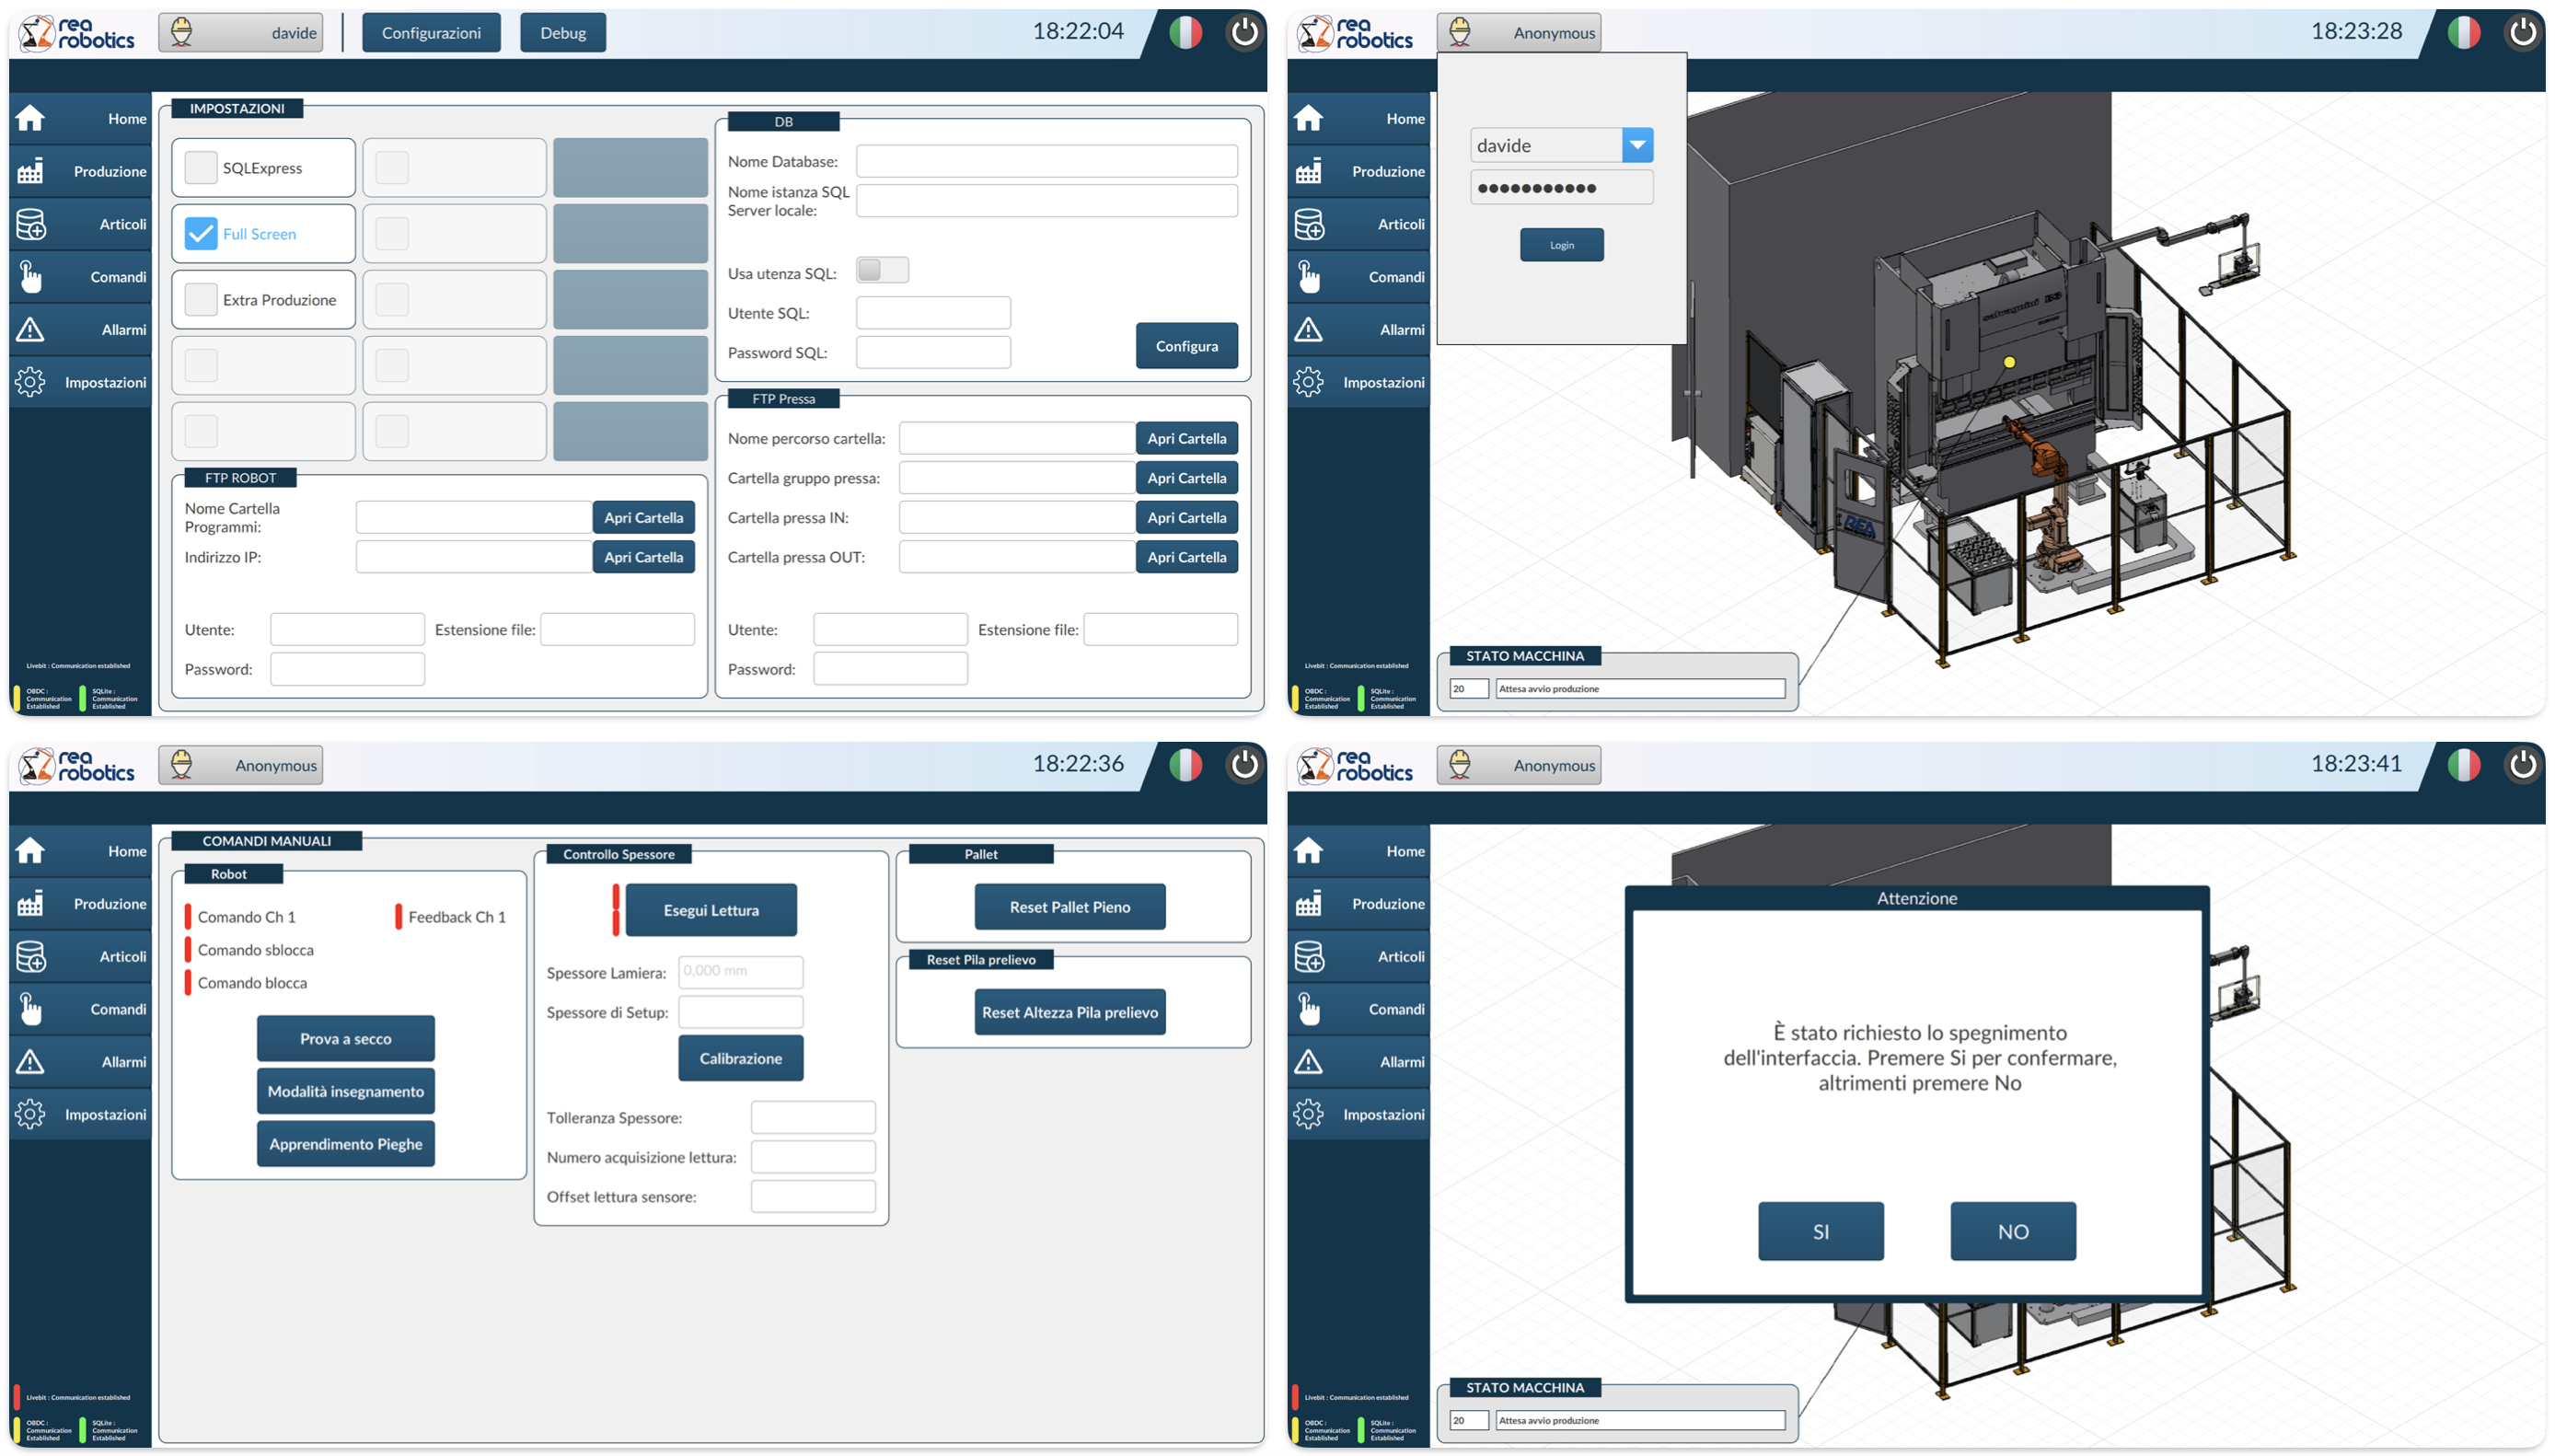
\includegraphics[width=1\linewidth]{Immagini/HMI01.png}
    \caption{4 illustrazioni dell'HMI}
    \label{fig:HMI01.png}
\end{figure}

\subsection{Considerazioni tecniche sulla risoluzione}
Grazie alla tecnologia responsive presente nativamente su FT Optix™, l'intero HMI è adattabile e scalabile su qualsiasi display, garantendo una corretta visualizzazione indipendentemente dalle dimensioni dello schermo. Tuttavia, poiché nel nostro caso lo SCADA è progettato per essere utilizzato principalmente su pannelli con risoluzione Full HD (1920x1080), è di fondamentale importanza che tutta l'interfaccia sia leggibile e fruibile dall'operatore senza barre di scorrimento laterali.
Considerando a maggior ragione che lo SCADA sarà utilizzato su dispositivi dotati di tecnologia touch in ambienti industriali, è cruciale che ogni elemento risulti chiaro, affidabile e di facile accesso. La leggibilità e la precisione dei comandi sono fondamentali per garantire la sicurezza e l'efficacia delle operazioni svolte dall'operatore in tali contesti.

\section{Gestione Database per la produzione}

Per quanto riguarda il database ho deciso di adottare diverse metodologie per la gestione dati. La prima esigenza dell'azienda è stata creare un ricettario per mantenere una serie di record con attributi ben specifici, e che permettesse l'integrazione e la comunicazione verso la scheda di produzione. La mia proposta di soluzione ideale è stata quella di suddividere il database in due tabelle: una completamente dedicata alla parte di \textit{Anagrafica articoli} presenti in macchina, e l'altra che riguardasse la \textit{Produzione}, in cui vengono registrati gli ordini. Questa rappresenta solo la prima fase di progettazione, poiché nello SCADA è necessario anche avere accesso ad altri dati, tra cui: lo \textit{Storico Produzioni}, che archivia tutte le produzioni completate, sia con esito positivo che negativo; tutte le variabili che potrebbero influire sull'integrità dello stato di un ordine (ad es: l'extra produzione); e tutti gli interventi effettuati tramite input all'HMI, come l'importazione e l'esportazione delle ricette. Infine, ho deciso di integrare all'HMI non solo il database locale creato da me, ma anche il SSMS fornito dall'azienda, per garantire maggiore flessibilità al sistema.

\subsection{Anagrafica Articoli} 
Questa sezione si occupa della gestione dell'inserimento di nuovi articoli da produrre nell'impianto. La progettazione ha richiesto due tipi di interventi: il primo ha riguardato la gestione del front-end dell'anagrafica; il secondo ha coinvolto la parte di back-end, con particolare attenzione a bottoni e gestione database. 

Il lavoro è iniziato con la creazione del menù, in particolare di un'interfaccia dedicata che possa integrare tutti i comandi necessari. Grazie a FT Optix™, è possibile implementare una sezione di inserimento dei singoli articoli composta dagli attributi richiesti dal sistema. In aggiunta, è stata predisposta una sezione di visualizzazione, che mostra tutti i dati del database, compresi gli attributi richiesti in precedenza. Per facilitare la gestione dei dati, è stato sfruttato un oggetto di tipo \textit{DataGridView}\textsuperscript{\cite{factorytalk_datagrid_example}}, che emula il funzionamento di una tabella, rendendo chiara e accessibile la consultazione dei dati. Dato che uno SCADA industriale deve gestire qualche centinaio di articoli, sono stati implementati sia un sistema di filtraggio dei prodotti in base a parametri specifici (selezionando gli attributi d'interesse), sia una barra di ricerca che permette di individuare rapidamente un prodotto già presente nel sistema. Inoltre, su richiesta, è stata aggiunta una sezione in basso (Figura: \ref{fig:AnagraficaArticoli.png}) per l'esportazione e l'importazione delle ricette, consentendo al sistema di caricare serie di articoli preconfigurati dal cliente, velocizzando e semplificando il processo di inserimento articoli.

\begin{figure} 
    \centering
    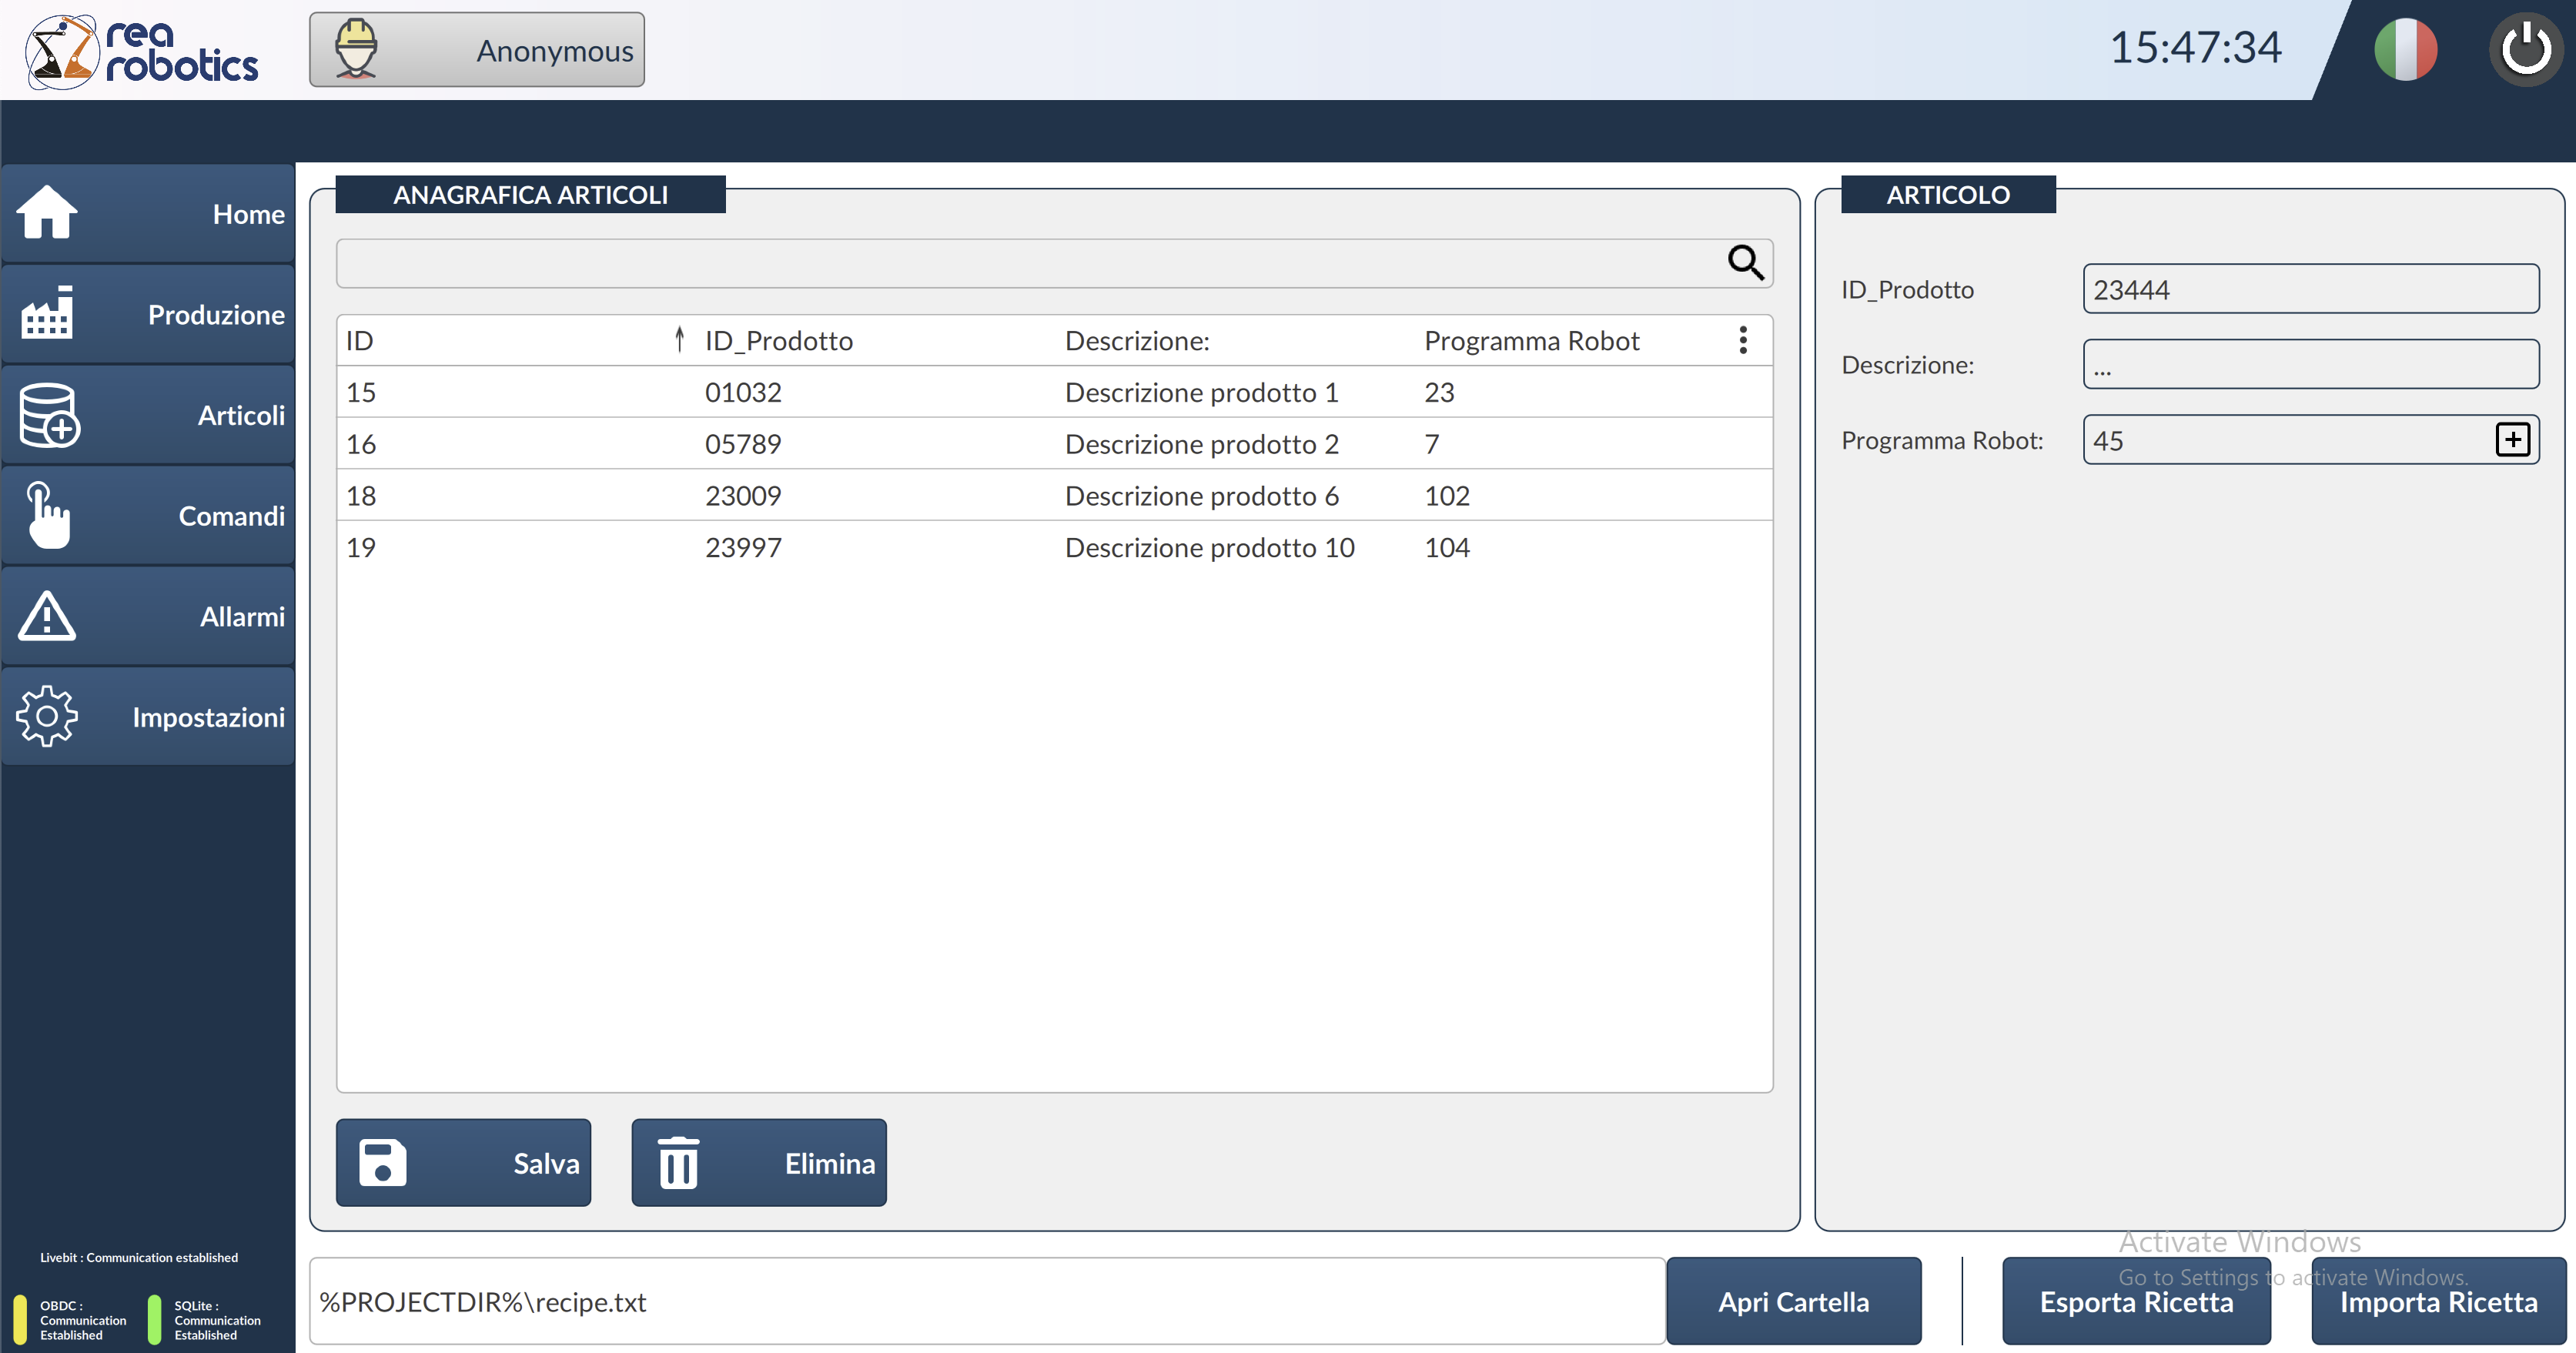
\includegraphics[width=1\linewidth]{Immagini/AnagraficaArticoli.png}
    \caption{Illustrazioni sezione \textit{Articoli}}
    \label{fig:AnagraficaArticoli.png}
\end{figure}

Per quanto riguarda la parte di back-end, il primo passo consiste nel configurare il database di riferimento. All'interno della Project View nella cartella DataStores deve essere creato un oggetto di tipo \textit{Embedded database}, che permette di importare un database \verb|.sqlite| su cui lavorare\textsuperscript{\cite{rockwelloptixdatastore}}. Successivamente, è necessario eseguire una serie di passaggi per poter impostare correttamente la struttura delle tabelle:

\begin{enumerate}
    \item Importare/impostare in \textit{Configuration} il nome del file del database da cui l'eseguibile dovrà estrarre i dati.
    \item Creare, tramite FT Optix™, le tabelle sotto il nome di \textit{RecipeSchema}, includendo tutti gli attributi di interesse necessari per la gestione delle ricette.
    \item Aprire il file creato, sotto il nome di \verb|filename.sqlite| tramite un software come DB4S, presente all'interno della cartella ApplicationFiles del programma, per impostare eventuali vincoli del database. Questo ultimo passaggio è facoltativo e può essere omesso qualora non siano richiesti vincoli specifici per i dati da raccogliere.
\end{enumerate} 

Prima di introdurre la sezione degli script in C\#, è importante chiarire due scelte di stile che ho adottato durante la progettazione del seguente database. Nel nostro caso ogni articolo deve essere caratterizzato da attributi ben definiti, che devono essere sempre presenti, indipendentemente dalla macchina su cui lo SCADA dovrà essere installato. In particolare:

\begin{itemize}
    \item \textbf{\textit{ID}}: un identificatore universale per il database, configurato come un intero, chiave primaria e auto-incrementale (\verb|INTEGER PRIMARY KEY AUTOINCREMENT|). Questo attributo permette ad ogni articolo di avere un identificativo distinto, senza mai ripetersi, nemmeno in caso di eliminazione o modifica di un prodotto. Questa scelta viene fatta per motivi di sicurezza, prevenendo eventuali conflitti di tuple in situazioni di sincronizzazione non corretta. 
    \item \textbf{\textit{Product\_ID}}: un identificatore specifico per il prodotto con vincoli meno restrittivi rispetto al primo. Questo campo non deve essere forzatamente un intero, bensì può essere anche un codice alfa-numerico, a discrezione del cliente. Come unici vincoli aggiunti, per non incorrere in errori di inserimento, ci sono l'unicità e l'obbligo di non essere nullo.
    \item \textbf{\textit{Robot\_Program}}: indica il programma che il robot dovrà utilizzare. Di norma, questi programmi sono identificati da numeri. Anche in questo caso, deve essere specificato il vincolo di obbligatorietà: non nullo, garantendo l'inserimento di un valore.
\end{itemize}
Partendo da questa base, è possibile inserire a piacimento ulteriori attributi in base alla necessità del cliente oppure dell'impianto su cui si sta lavorando, ripetendo i passaggi descritti precedentemente. 
L'altra considerazione da fare riguarda l'uso dei \textit{RecipeSchema} in FT Optix™, per cui esistono alcuni vincoli dati dal software: ad esempio, l'obbligo di anteporre il carattere \verb|/| a tutti gli attributi creati sia nel database locale sia in interfaccia. Inoltre, FT Optix™ supporta nativamente, attraverso le API, solo operazioni di base per le ricette, quali: INSERT, UPDATE, DELETE e SELECT\textsuperscript{\cite{rockwelloptixsqlquery}}. Sebbene inizialmente questo possa sembrare un vantaggio, dato che permette un accesso semplificato tramite i tool integrati, in alcuni casi può rappresentare una limitazione se si desidera interagire attraverso funzioni più complesse con il database. Per questo motivo, FT Optix™ fornisce la possibilità di creare in prima persona script in C\#, dando piena flessibilità e controllo diretto sul database al programmatore. Questa scelta si è dimostrata vincente, perchè mi ha permesso di creare script unici per la successiva gestione dei dati. 


Per quanto riguarda invece la parte di back-end, iniziamo con l'inserimento degli articoli nel database. Utilizzando i \textit{RecipeSchema}\textsuperscript{\cite{factorytalk_recipes}}, FT Optix™ mette a disposizione un oggetto \textit{RunTimeNetLogic}\textsuperscript{\cite{factorytalk_netlogic}} di tipo \textit{RecipeController}, che include già una serie di funzioni di base. Nel nostro caso, è necessario implementare all'interno del file \verb|RecipeController.cs| uno script che permetta l'inserimento di un prodotto in Anagrafica correttamente. In Visual Studio, creiamo quindi una funzione che verrà richiamata dal tasto SALVA presente nell'interfaccia. Per prima cosa, scriviamo il comando \verb|[ExportMethod]|(riga 2) che consente di rendere accessibile la funzione direttamente in FT Optix™ (questa pratica verrà ripetuta anche per futuri script). Successivamente, definiamo la funzione specificando gli attributi in input che ci interessa salvare. All'interno del codice, viene richiamato il database locale (oppure SSMS) tramite \verb|myStore| e la tabella di interesse \verb|myTable| (rispettivamente righe 8-9). Da qui possiamo utilizzare la funzione \verb|.Insert| di FT Optix™, con i valori precedentemente richiamati, per popolare il database (riga 18).
\begin{csharp}
...
    [ExportMethod]
    public void Insert_Product_in_Anagrafica(string Product_ID, string Descr, int Robot_Program)
    {
        try
        {
            // Inserimento nella tabella
            var myStore = Project.Current.Get<Store>("DataStores/EmbeddedDatabase1");
            var myTable = myStore.Tables.Get<Table>("RecipeSchema1");
            string[] columns = { "Name", "/Descr", "/Robot_Program", "/Product_ID" };
            var values = new object[1, 4];
            values[0, 0] = Product_ID;
            values[0, 1] = Descr;
            values[0, 2] = Robot_Program;
            values[0, 3] = Product_ID;
    
            // Eseguire la query di inserimento
            myTable.Insert(columns, values);
    
            // Se l'operazione è andata a buon fine
            Log.Info("RecipeSchema1", "Inserimento riuscito: " + values[0, 1]);
        }
        catch (Exception ex)
        {
            // In caso di errore, viene catturata l'eccezione e viene stampato il messaggio d'errore
            Log.Error("RecipeSchema1", "Errore durante l'inserimento: " + ex.Message);
            popup.OpenPopUp(ex.Message, 0);
        }
    }
...
\end{csharp}
Due aspetti importanti meritano attenzione in questa fase. In primo luogo, si osserva la presenza del carattere \verb|/| negli attributi, come richiesto dalle specifiche di FT Optix™ per le ricette. In secondo luogo, vi è un attributo \verb|Name|, il quale rappresenta un vincolo essenziale nella costruzione delle ricette in FT Optix™; nel nostro caso, assegniamo a tale campo un valore a scelta tra quelli disponibili. Inoltre, la funzione è stata inserita in un blocco \verb|try-catch| per garantire maggiore controllo su eventuali errori di inserimento in FT Optix™ (altra pratica ampliata anche ad altri script, come regola di buona programmazione).
Ora passiamo ad un'ulteriore richiesta che riguarda le importazioni di articoli esterni. In questo caso, è stato necessario avvalerci di un ulteriore oggetto, \textit{RunTimeNetLogic}, direttamente associato alla tabella, al fine di implementare una funzione capace di controllare un file esterno definito come \verb|dati.txt|. Di seguito è riportato il codice:
\begin{csharp}
...
    // Metodo per controllare e leggere il file
    private static void ControllaFile(Object source, ElapsedEventArgs e)
    {
        // Specifica la cartella e il nome del file
        string cartella = @"C:\Users\davide.quartucci\Desktop\InserimentoAnagraficaSuDB";
        string nomeFile = "dati.txt";
    
        // Cerca il file nella cartella specificata
        string percorsoFile = Path.Combine(cartella, nomeFile);
    
        if (File.Exists(percorsoFile))
        {
            try
            {
                // Leggi il contenuto del file
                string[] righe = File.ReadAllLines(percorsoFile);
    
                foreach (string riga in righe)
                {
                    try
                    {
                        // Dividi la riga in tre parti usando il separatore ';'
                        string[] campi = riga.Split(';');
    
                        if (campi.Length != 3)
                        {
                            throw new FormatException("La riga non contiene esattamente 3 campi.");
                        }
    
                        // Assegna i campi a variabili locali
                        string Product_ID = campi[0];
                        string Descr = campi[1];
                        int Robot_Program;
    
                        // Prova a convertire il terzo campo in un intero
                        if (!int.TryParse(campi[2], out Robot_Program))
                        {
                            throw new FormatException("Il campo Robot_Program non è un intero valido.");
                        }
    
                        //Esegue l'inserimento nel DB di una nuova anagrafica
                        var myStore = Project.Current.Get<Store>("DataStores/EmbeddedDatabase1");
                        var myTable = myStore.Tables.Get<Table>("RecipeSchema1");
                        string[] columns = { "Name", "/Descr", "/Robot_Program", "/Product_ID" };
                        var values = new object[1, 4];
                        values[0, 0] = Product_ID;
                        values[0, 1] = Descr;
                        values[0, 2] = Robot_Program;
                        values[0, 3] = Product_ID;
                        myTable.Insert(columns, values);
                    }
                    ... // Gestione eccezioni ed eliminazione file dopo la lettura
\end{csharp}
Nel codice appena illustrato viene richiamata la seguente funzione: \verb|dati.txt| situato in un percorso preimpostato (righe 6-7). La scelta di definire un percorso ben specifico è stata fatta per evitare problemi imprevisti durante l'inserimento dei dati. La funzione prosegue analizzando le righe del file, secondo le specifiche \textit{Product\_ID; Descrizione; Robot\_Program} (righe da 17 a 37). A partire da riga 42, il codice procede con l'inserimento all'interno del database di tutti i dati del file, e infine, lo elimina come richiesto. Ovviamente, questa funzione deve essere richiamata ciclicamente per garantire un aggiornamento continuo del database, facilitando così, ad esempio, la trasmissione di nuovi articoli dagli uffici di produzione direttamente alla macchina. Per automatizzare l'intero processo, nel metodo \verb|Start| (creato nativamente da FT Optix™) ho deciso di configurare un timer che ogni 10 secondi ripete l'operazione di lettura ed importazione degli articoli nell'anagrafica, assicurando aggiornamento costante e sincronizzazione dei dati:
\begin{csharp}
...
    private static Timer timer; // Timer per eseguire l'operazione ogni 10 secondi

    public override void Start()
    {
        // Insert code to be executed when the user-defined logic is started
        
        // Imposta e avvia il timer
        timer = new Timer(10000); // 10000 millisecondi = 10 secondi
        timer.Elapsed += ControllaFile; // Associa l'evento Elapsed all'handler
        timer.AutoReset = true; // Ripeti l'operazione ogni 10 secondi
        timer.Enabled = true; // Abilita il timer
    }
...
\end{csharp}
Per tutte le altre funzionalità, come l'eliminazione di articoli, ricerche ed importazioni/esportazioni da HMI, sono state sfruttate funzionalità di base già presenti nel programma. Il lavoro si è concentrato sull'ampliamento e personalizzazione di questi strumenti affinché si integrassero correttamente con il sistema.

\subsection{Ordini di Produzione}

Questa sezione si focalizza sulla fase di produzione degli articoli, con focus sull'inserimento, l'avvio e la gestione di una nuova produzione. La progettazione ha seguito il medesimo approccio adottato per la sezione dell'anagrafica. Per quanto riguarda l'interfaccia, ho preferito dividere la creazione di un nuovo ordine di produzione dalla gestione della produzione stessa, poiché nel monitoraggio è necessario tenere in primo piano molti più attributi rispetto alla sezione di anagrafica. Dal punto di vista progettuale, troviamo ancora un oggetto di tipo \textit{DataGridView}, che anche in questo caso serve per tenere sotto controllo lo stato degli ordini. Infatti, è stato anche configurato in modo che cambi colore in base allo stato dell'ordine: verde per gli articoli che sono attualmente in produzione, giallo per quelli in attesa e rosso per eventuali interruzioni impreviste. Anche in questa sezione è stato implementato un sistema di filtraggio, mentre nella parte inferiore della schermata troviamo un pannello che tiene sotto controllo lo stato/passo in cui si trova la macchina (il suo funzionamento verrà illustrato nella sezione \ref{sec:Sviluppo back-end e integrazione con il PLC}). Sempre nella parte inferiore della schermata, inoltre, sono presenti i pulsanti che permettono la gestione degli ordini di macchina. Prima di procedere alla fase implementativa, è stato progettato anche un popup per \textit{Nuova Produzione} (Figura:\ref{fig:Produzione.png}), che permette di inserire gli ordini in database. Questo popup è una finestra che richiede le specifiche di produzione, ovvero:
\begin{itemize}
    \item \textit{\textbf{Ordine di Produzione}}: identificativo dell'ordine, configurato come campo testuale.
    \item \textit{\textbf{Nome Articolo}}: mostra a schermo un menù a tendina che consente di selezionare il \textit{Product\_ID} dell'articolo già presente in database, ereditando tutte le caratteristiche definite nella sezione Anagrafica.
    \item \textit{\textbf{Quantità\_Richiesta}}: è la quantità dell'ordine da produrre inizialmente.
\end{itemize}

\begin{figure} 
    \centering
    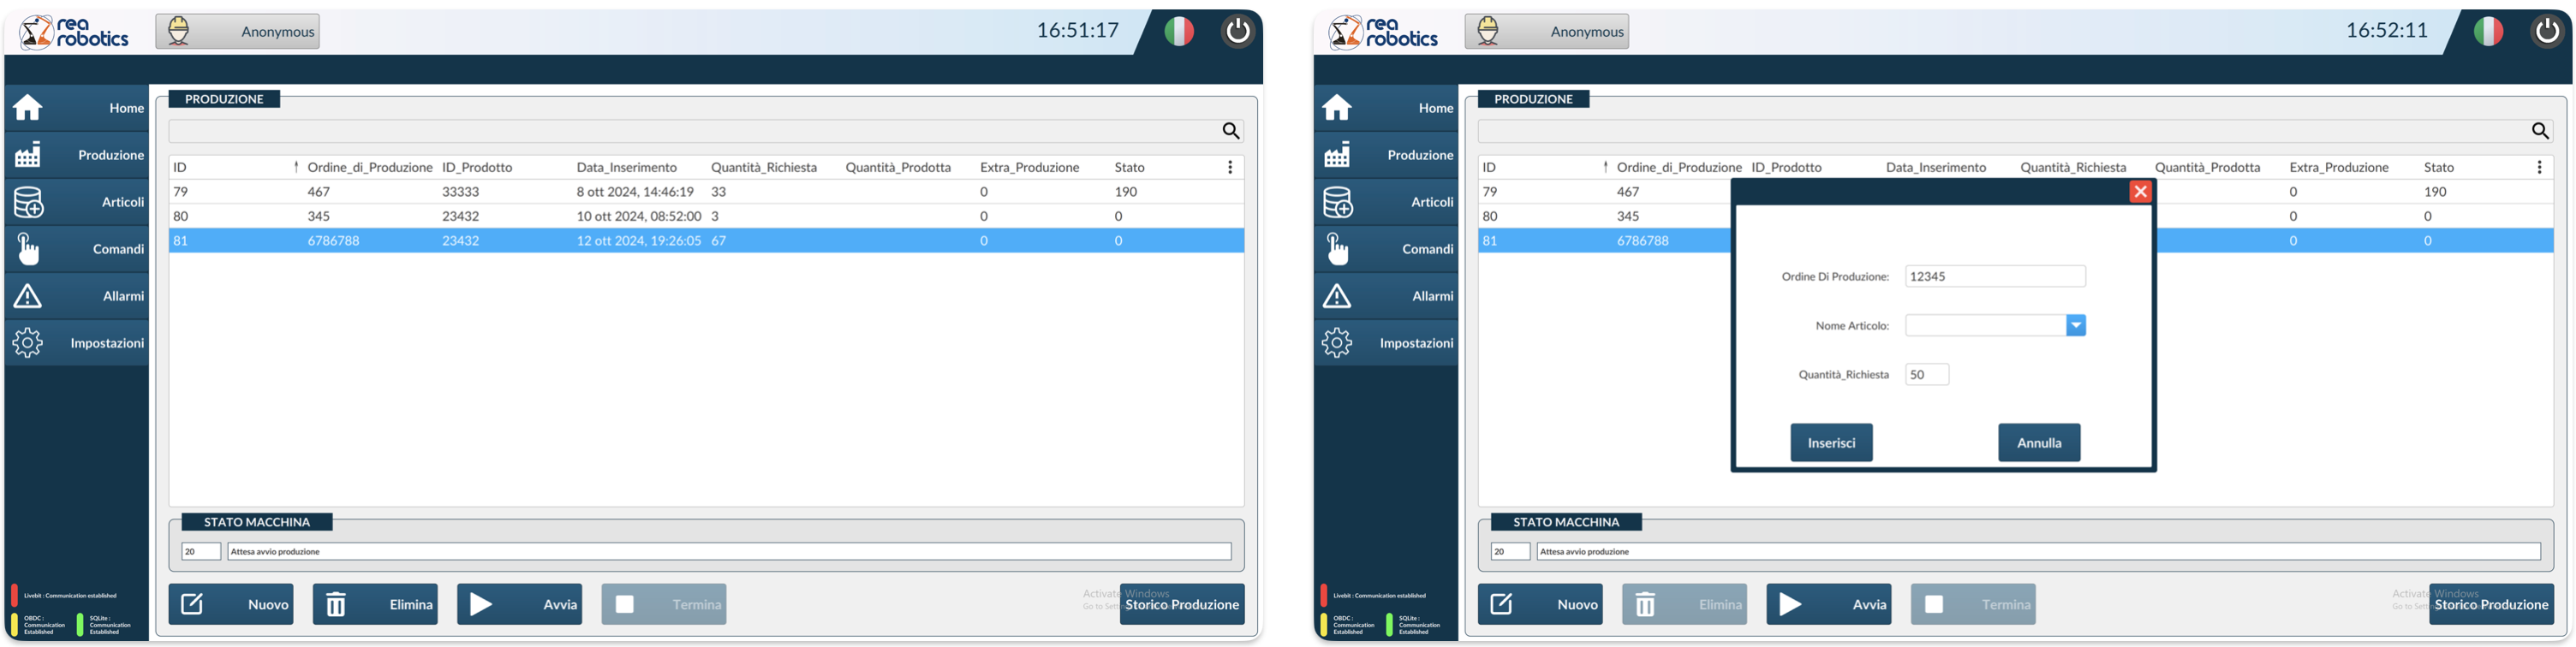
\includegraphics[width=1\linewidth]{Immagini/Produzione.png}
    \caption{Illustrazioni sezione \textit{Produzione} e sottosezione \textit{Nuova Produzione}}
    \label{fig:Produzione.png}
\end{figure}

Fatto questo, ulteriori attributi vengono impostati durante l'inserimento dell'ordine. Infatti, dopo aver specificato i dati precedenti e premuto il tasto "inserisci", viene richiamata una funzione all'interno di \verb|RecipeController.cs|, sviluppata seguendo le stesse linee guida di quella già analizzata in Anagrafica. In questo caso, poiché la produzione necessita di parametri aggiuntivi, come ad esempio: \textit{Date\_Insert, Status, Extra\_Production, ...}, questi attributi vengono inizialmente impostati su valori predefiniti. Un attributo che necessita di analisi è la Data di Inserimento (gestita a riga 16). Qui viene utilizzato \verb|DateTime.Now| per ottenere il momento esatto del salvataggio, con successivo parsing in \verb|.ToString|, come richiesto per il corretto inserimento dei dati nel database.

\begin{csharp}
...
[ExportMethod]
public void Insert_newProduction(string Odp, string NomeArticolo, int quantità)   
{
    try
    {
        // Inserimento nella tabella
        var myStore = Project.Current.Get<Store>("DataStores/EmbeddedDatabase1");
        var myTable = myStore.Tables.Get<Table>("RecipeSchema2");
        string[] columns = { "Name", "/Odp", "/NomeArticolo", "/Date_Insert", "/Quantità", "/Extra_Production", "/Total_Reject", "/Status" };
        var values = new object[1, 8];

        values[0, 0] = Odp;
        values[0, 1] = Odp;
        values[0, 2] = NomeArticolo;
        values[0, 3] = DateTime.Now.ToString("yyyy-MM-ddTHH:mm:ss.fffffffK"); 
        values[0, 4] = quantità;
        values[0, 5] = 0;
        values[0, 6] = 0;
        values[0, 7] = 0;

        // Eseguire la query di inserimento
        myTable.Insert(columns, values);

        // Se l'operazione è andata a buon fine
        Log.Info("RecipeSchema2", "Inserimento riuscito: " + values[0, 1]);
    }
    catch (Exception ex)
    {
        // In caso di errore, viene catturata l'eccezione e viene stampato il messaggio d'errore
        Log.Error("RecipeSchema2", "Errore durante l'inserimento: " + ex.Message);
        popup.OpenPopUp(ex.Message, 0);
    }
}
...
\end{csharp}

Prima di passare all'implementazione della funzione \textit{Avvia Produzione}, è necessario soffermarci su un'ulteriore richiesta da parte dell'azienda: la gestione di un'eventuale \textit{Extra Produzione} per rispondere a esigenze particolari di produzione. Per questo motivo, sono stati attuati 2 passaggi:
\begin{enumerate}
    \item Assicurarsi che l'\textit{extra produzione} sia sempre disponibile e attivabile su richiesta tramite un'opzione accessibile solamente dal programmatore.
    \item Nel caso in cui sia attiva, permettere alla macchina di poterla gestire lato back-end (che verrà approfondito nella sezione \ref{sec:Sviluppo back-end e integrazione con il PLC}).
\end{enumerate}
Per il primo punto la soluzione adottata consiste nell'inserire all'interno della sezione \textit{Impostazioni} un interruttore \textit{Extra Produzione}, attivabile esclusivamente in modalità sviluppatore o con le opportune autorizzazioni\textsuperscript{\cite{factorytalk_users_groups}}. Fatto questo è stato progettato un popup che appare al termine di ogni ciclo di produzione e, tramite un menù, chiede se si vogliono produrre ulteriori componenti, permettendo così alla macchina di riavviare il ciclo produttivo (Figura:\ref{fig:Extraproduzione.png}).

\begin{figure} 
    \centering
    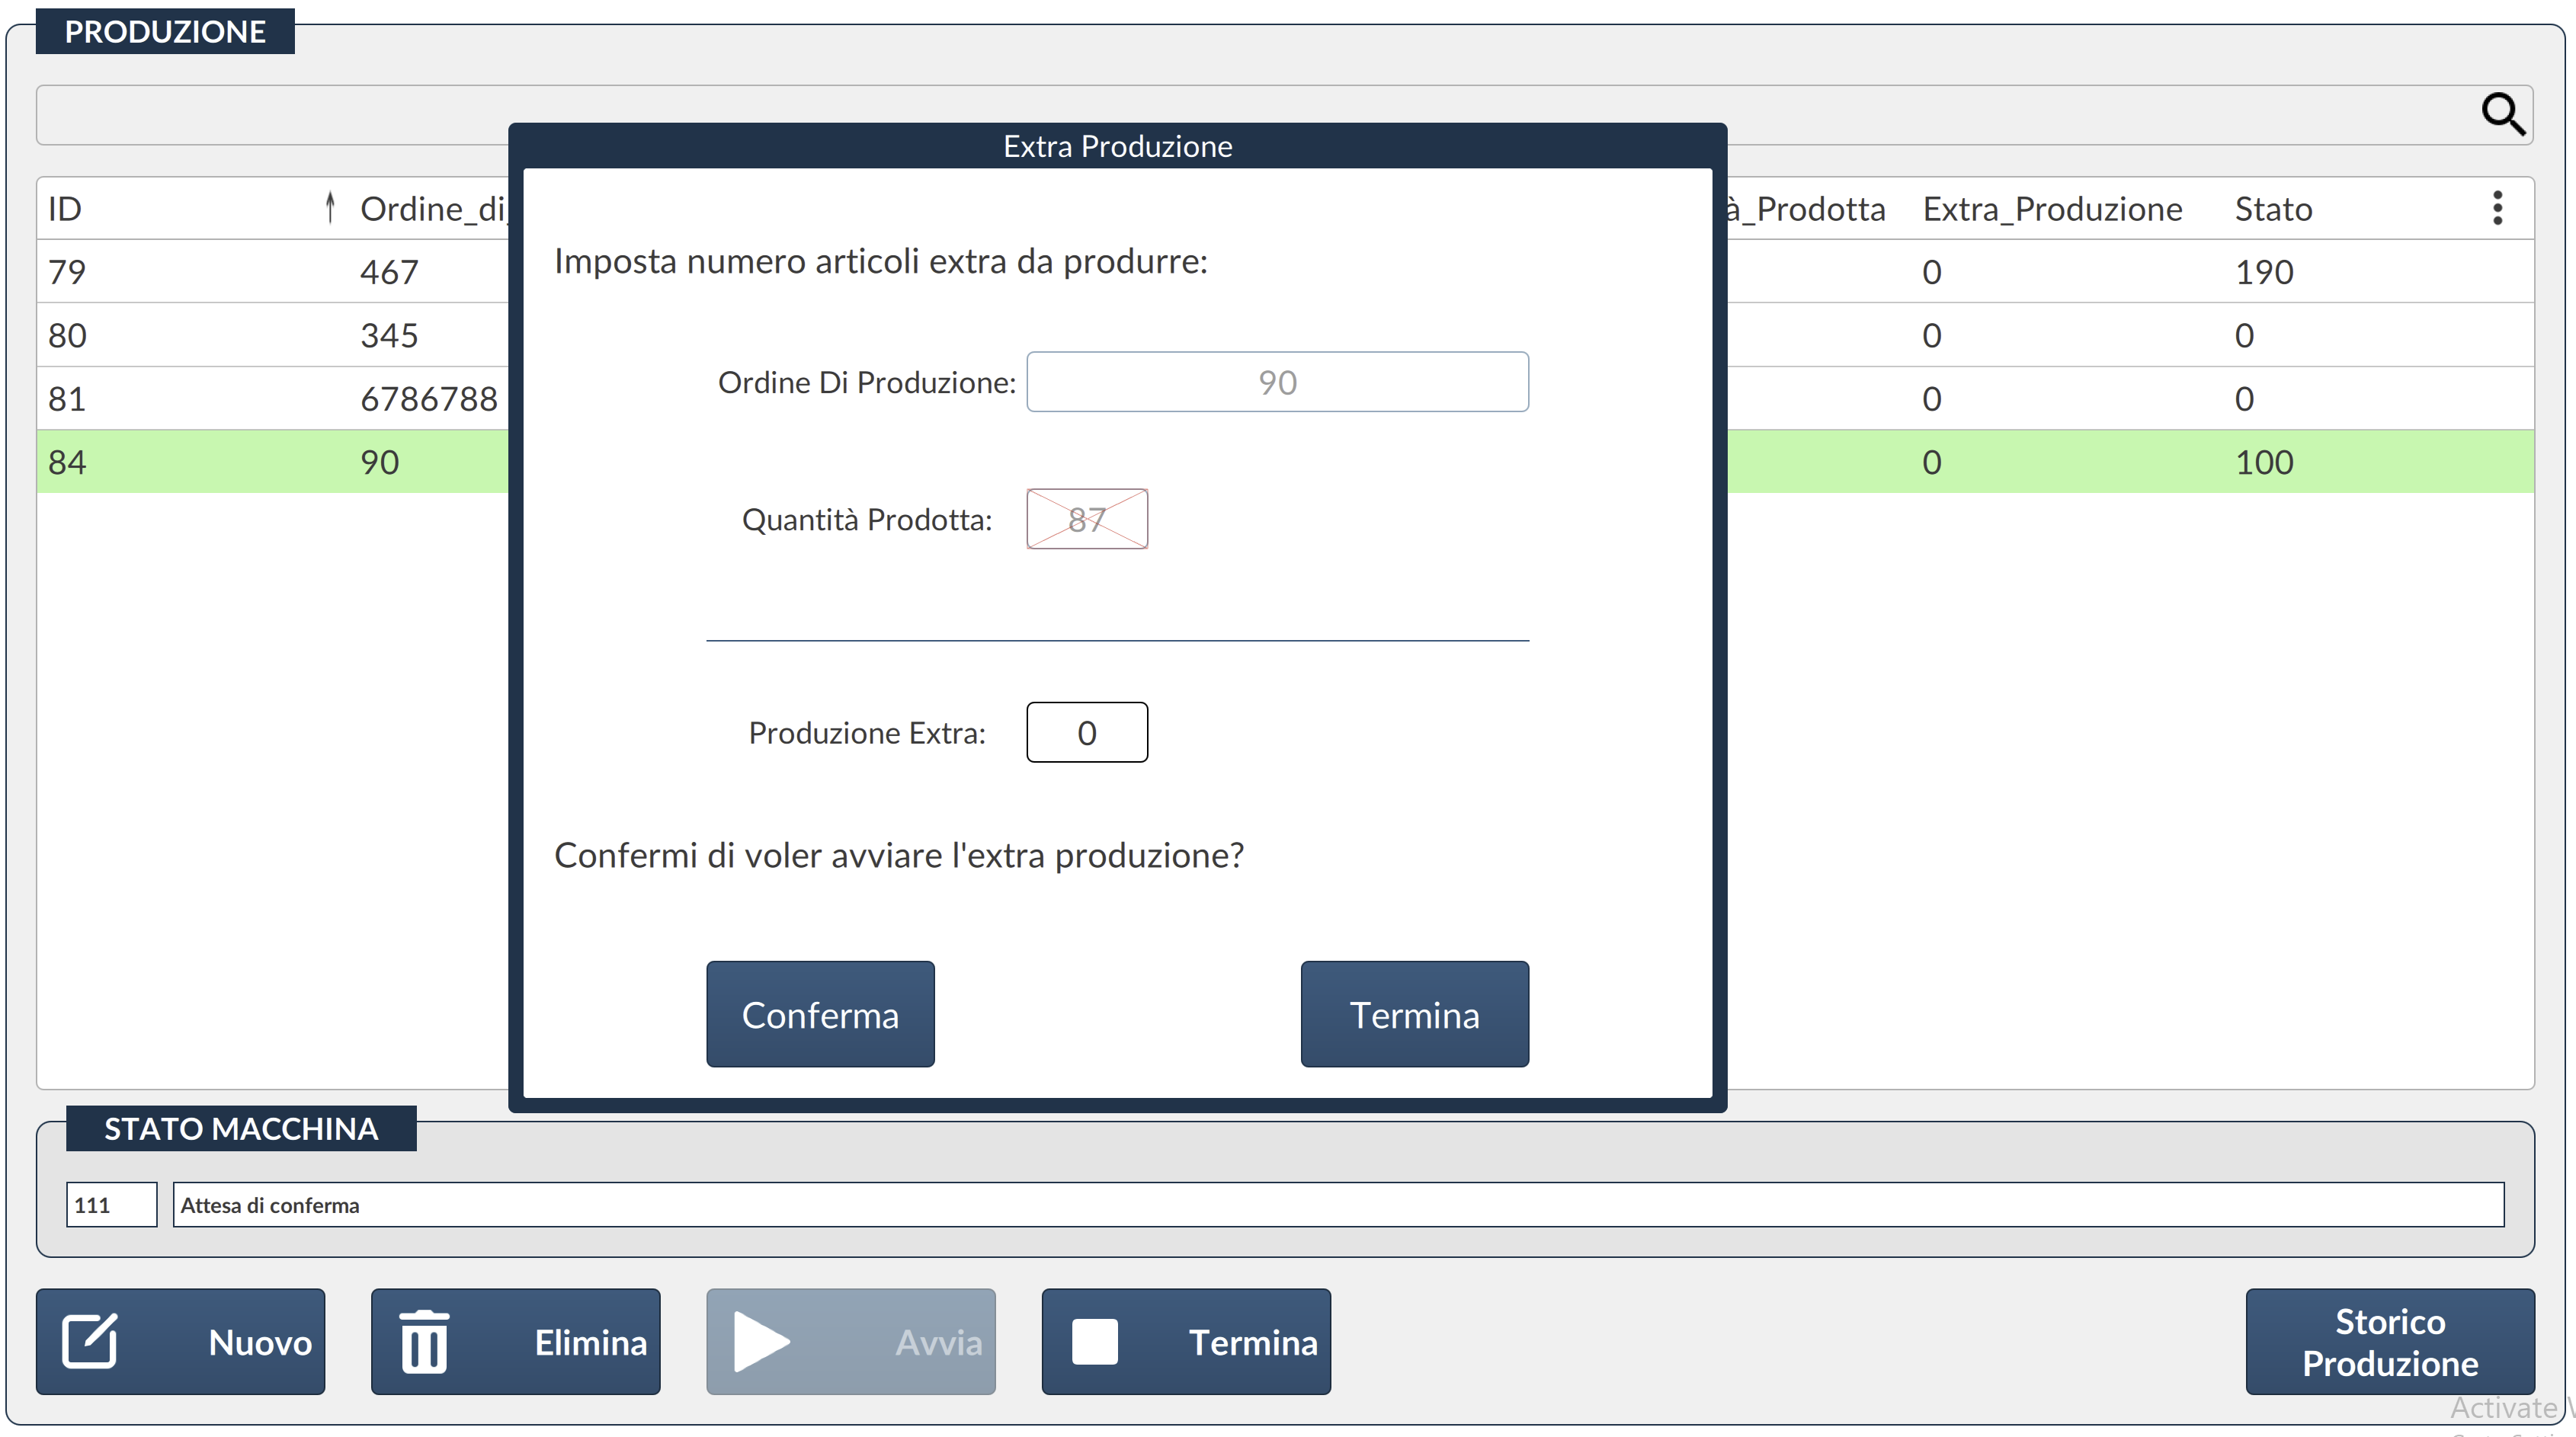
\includegraphics[width=1\linewidth]{Immagini/ExtraProduzione.png}
    \caption{Esempio richiesta di \textit{Extra Produzione}}
    \label{fig:Extraproduzione.png}
\end{figure}

Passiamo ora a due iterazioni principali nello SCADA: \textit{Avvia Produzione} e \textit{Termina Produzione}. Nel caso di \textit{Avvia Produzione}, dopo aver dato conferma tramite apposito popup di verifica, viene richiamata la funzione \verb|pr_AvviaLocale|, che si occupa di configurare in autonomia le variabili fondamentali della produzione, permettendo alla macchina a stati di poterne usufruire:

\begin{csharp}
...
    /// <summary>
    /// Avvia produzione
    /// </summary>
    [ExportMethod]
    public void pr_AvviaLocale(long id)
    {
        Project.Current.GetVariable(VariablePaths.PathOdlStart).Value = id;
        Project.Current.GetVariable(VariablePaths.Pathap_start).Value = true;
    }
...
\end{csharp}

Per quanto riguarda \textit{Termina Produzione} invece, viene semplicemente impostata la variabile \verb|pr_ButtonTerminaSelected = TRUE|, invocando la macchina a stati. Quest'ultima, nel passo corrispondente, richiama la funzione \verb|pr_TerminateAllRunningLocale|, che si occupa per spostare l'ordine nello storico della produzione. Nella funzione indicata e successivamente illustrata, il sistema procede dapprima ad individuare l'ordine con lo stato 160 "di aggiornamento tabelle e spostamento nello storico" (righe 8-9). Poi, una volta trovato l'ordine, viene creato un nuovo oggetto temporaneo in cui vengono inseriti tutti gli attributi dell'ordine, con l'aggiunta della data di terminazione della produzione (da riga 17 a riga 25). Infine, l'oggetto risultante viene trasferito nella tabella di \textit{Storico Produzione} (riga 28).

\begin{csharp}
...
    /// <summary>
    /// Recupera i dati delle produzioni terminate e li sposta nello storico
    /// </summary>
    public void pr_TerminateAllRunningLocale()
    {
        object[,] result;
        _store = Project.Current.Get<Store>(DATASTORE_DATABASE);
        _store.Query($"SELECT * FROM {TABLE_NAME} WHERE \"/Status\" = 160", out _, out result);
    
        if (result.GetLength(0) == 0 || result.GetLength(1) == 0)
        {
            Log.Warning("pr_TerminateAllRunning no record found");
            return;
        }
    
        ReaToClienteLocale prod = new ReaToClienteLocale();
        prod.Production_Command = "" + result[0, 0];
        prod.Product_ID = (string)result[0, 3];
        prod.dt_start = (DateTime?)result[0, 4];
        prod.dt_end = DateTime.Now;
        prod.Quantity_Requested = (long)result[0, 8];
        prod.Quantity_Produced = (long)result[0, 9];
        prod.Total_Reject = (long)result[0, 11];
        prod.Extra_Production = (long)result[0, 10];
    
        _storicoprod = new RuntimeNetLogicReaToClienteStoricoLocale();
        _storicoprod.sp_InsertLocale(prod);

    }
...
\end{csharp}

\subsection{Storici Produzione/Allarmi}
Lo storico di produzione risulta accessibile tramite pulsante apposito, inserito nell'interfaccia di \textit{Produzione}. Al suo interno è stata progettata un'interfaccia simile a quella di \textit{Produzione}, ma con alcune differenze. Nello specifico, non è presente nessun pulsante per l'interazione diretta con la macchina, ma solo un \textit{DataGridView} che mostra tutte le informazioni sugli ordini prodotti. Difatti, le uniche iterazioni disponibili avvengono tramite un filtro di ricerca simile a quelli già trattati in precedenza, con l'aggiunta della possibilità di effettuare ricerche basate su data, o su un determinato periodo di tempo. La popolazione di questa tabella avviene solamente tramite la funzione analizzata nella sezione precedente, seguendo pressoché lo stesso approccio utilizzato per l'interfaccia di \textit{produzione}. Per quanto riguarda la parte back-end, è stato dapprima creato un \textit{RecipeSchema} contenente gli attributi necessari e, successivamente, sulla base del \verb|RuntimeNetLogic| fornito, è stata implementata la funzione di inserimento nel database \verb|sp_InsertLocale|. Questa funzione, come già descritto nelle sezioni precedenti, si occupa di inserire l'oggetto \verb|prod|, completo di tutti i suoi attributi nella tabella dello storico.

\begin{figure} 
    \centering
    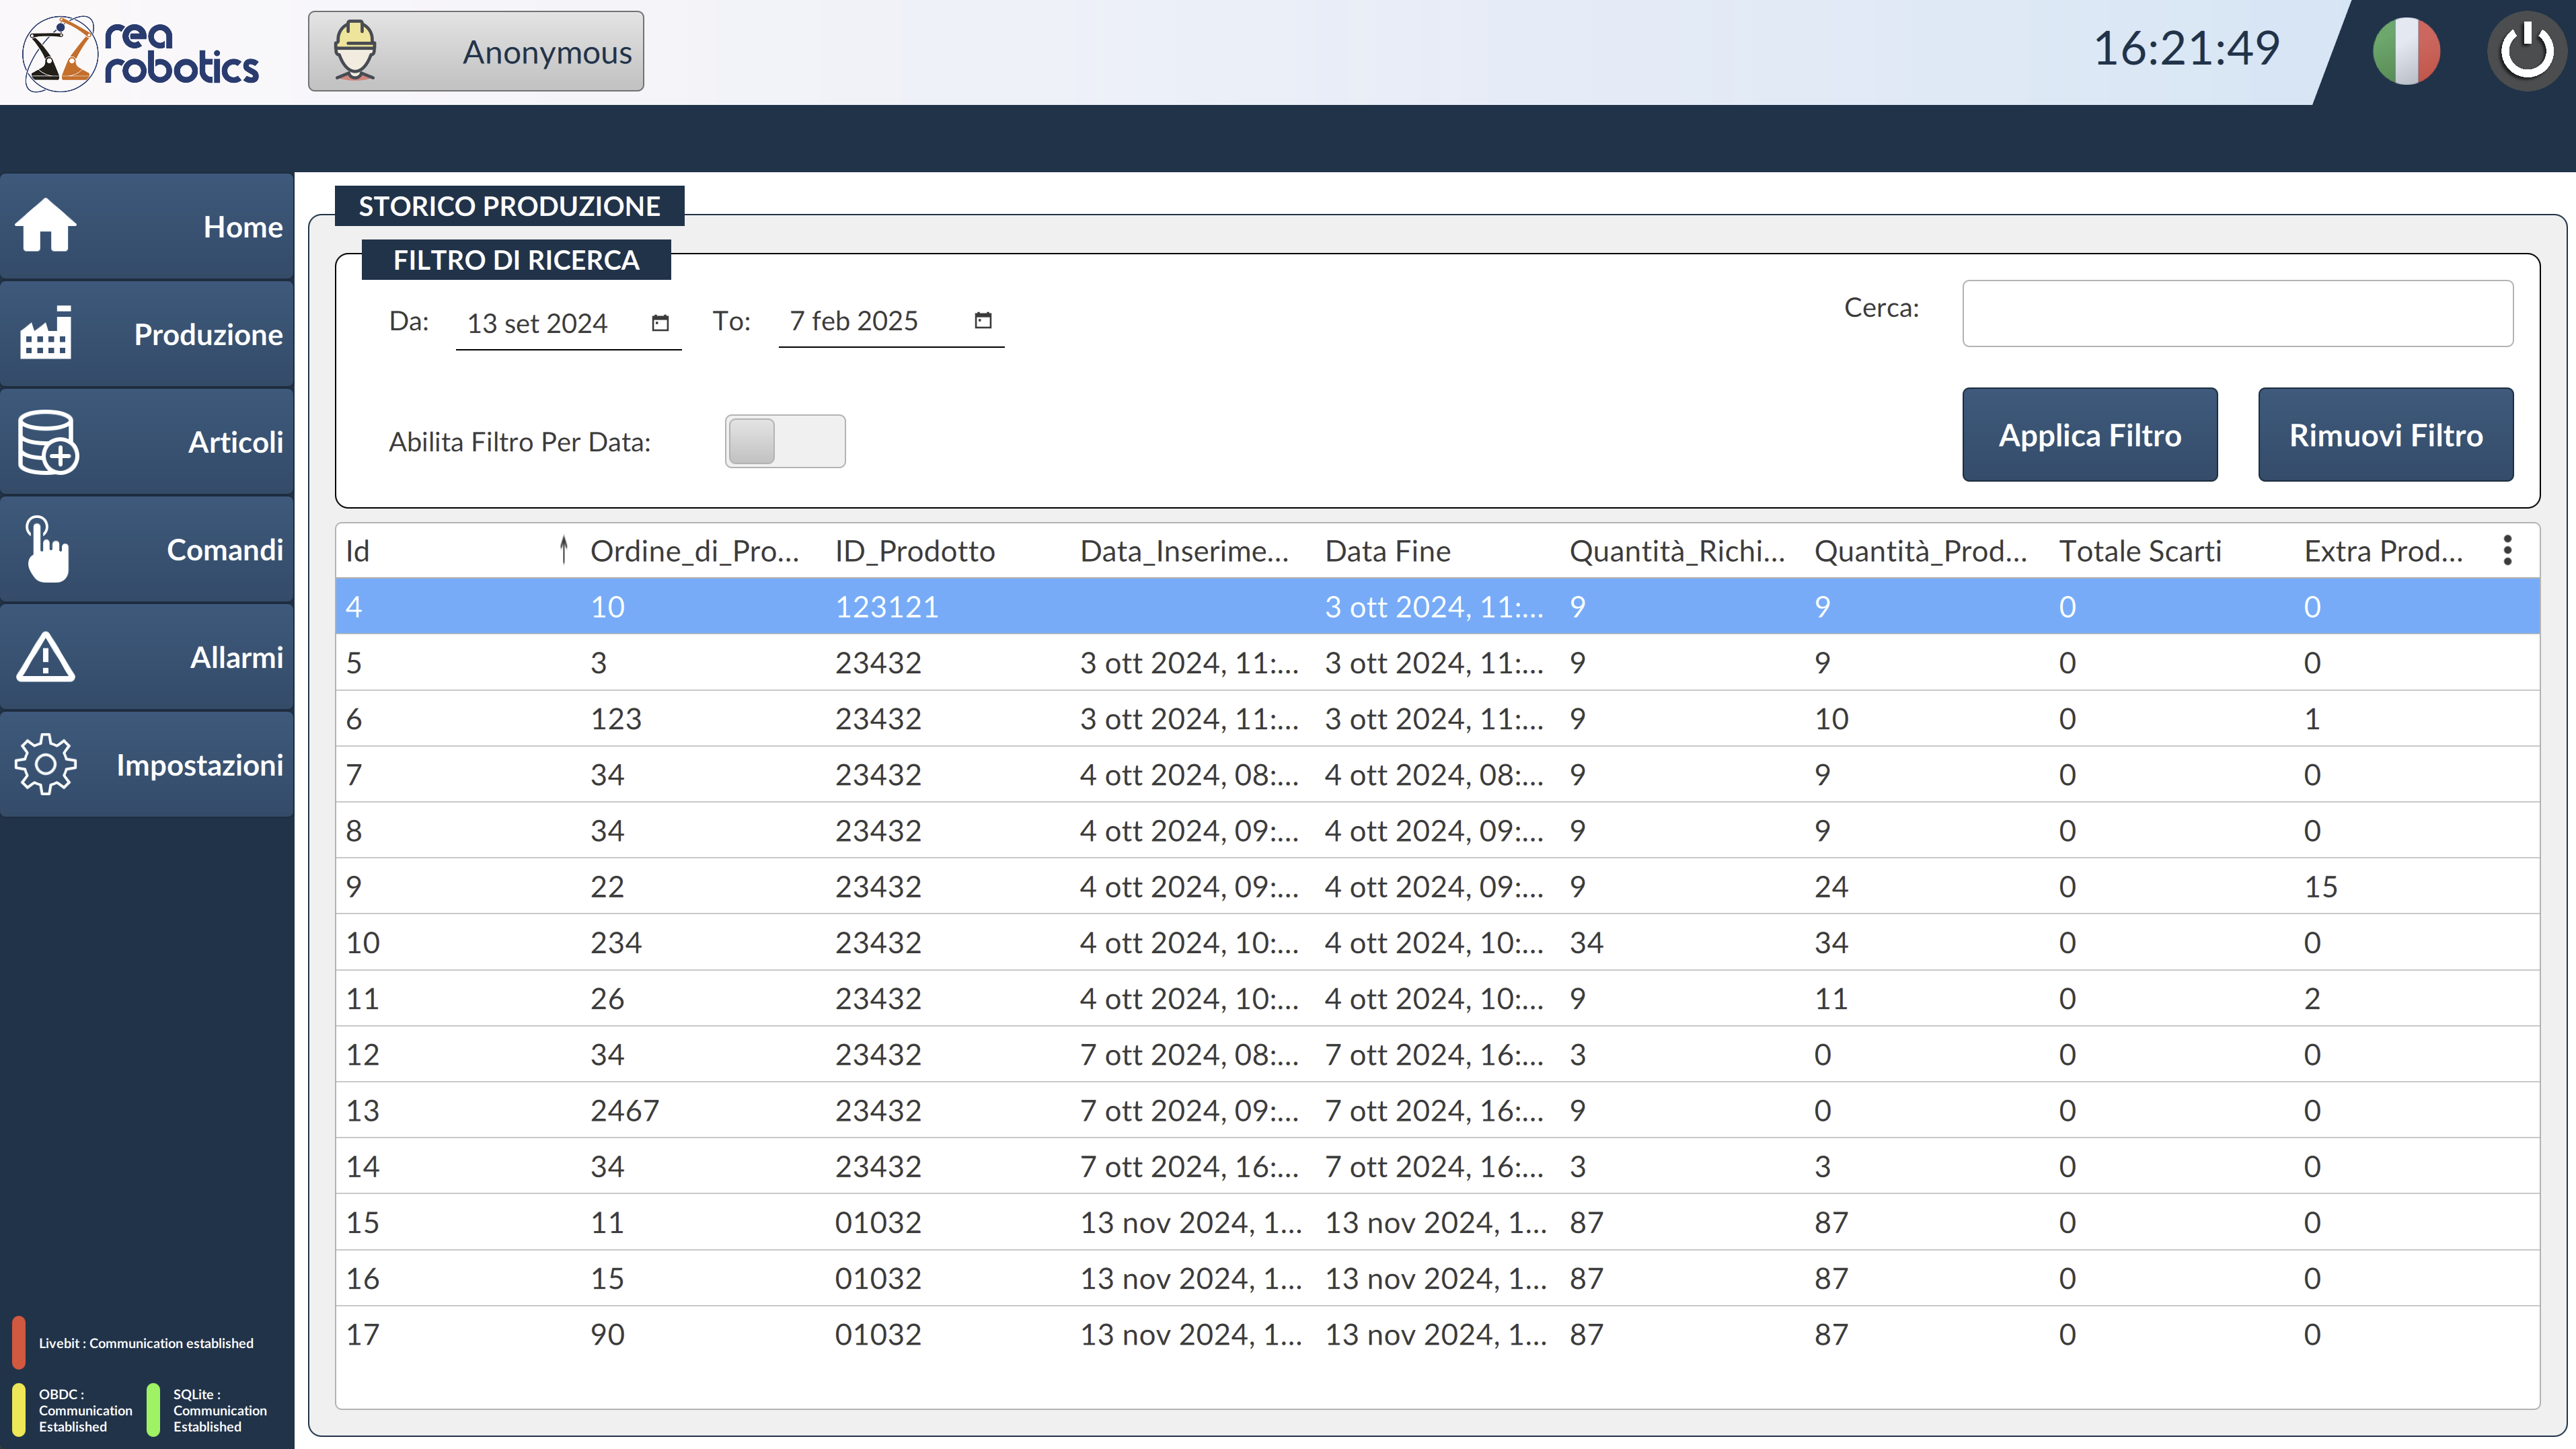
\includegraphics[width=1\linewidth]{Immagini/StoricoProduzione.png}
    \caption{Illustrazione sezione \textit{Storico Produzione}}
    \label{fig:StoricoProduzione.png}
\end{figure}

\begin{csharp}
...
public class RuntimeNetLogicReaToClienteStoricoLocale : BaseNetLogic
{
    ... //Altro codice fornito da FT Optix

    /// <summary>
    /// Inserisce un record nello storico
    /// </summary>
    public void sp_InsertLocale(ReaToClienteLocale prod)
    {
        try
        {
            string[] columns = { "/Production_Command", "/Product_ID", "/dt_start", "/dt_end", "/Quantity_Requested", "/Quantity_Produced", "/Total_Reject", "/Extra_Production" };

            var values = new object[1, 8];
            values[0, 0] = prod.Production_Command;
            values[0, 1] = prod.Product_ID;
            values[0, 2] = prod.dt_start;
            values[0, 3] = prod.dt_end;
            values[0, 4] = prod.Quantity_Requested;
            values[0, 5] = prod.Quantity_Produced;
            values[0, 6] = prod.Total_Reject;
            values[0, 7] = prod.Extra_Production;

            _store = Project.Current.Get<Store>(DATASTORE_DATABASE);
            _table = _store.Tables.Get<Table>(TABLE_NAME);
            _table.Insert(columns, values);

        }
        catch (Exception ex)
        {
            Log.Warning($"ERROR: sp_InsertLocale {ex.Message}");
        }
    }

}
...
\end{csharp}

Per quanto riguarda la gestione degli allarmi\textsuperscript{\cite{factorytalk_alarms}}, ci sono diversi aspetti da analizzare. Innanzitutto, dal punto di vista progettuale sono stati creati due pannelli dedicati: uno per la visualizzazione della lista di allarmi e un altro per i warning attivi. Di seguito, la schermata rimane essenziale, includendo solamente i pulsanti per la gestione di alcuni allarmi e warning, oltre alla sezione di \textit{Storico Allarmi}. A differenza di altre sezioni, gli allarmi non vengono gestiti tramite database ma direttamente da FT Optix™. Infatti, all'interno della cartella di progetto è presente una sotto-cartella dedicata a contenere solamente allarmi e warning (\ref{fig:CartellaAllarmi.png}) dell'impianto. 

\begin{figure}[!ht]
    \centering
    \begin{subfigure}[t]{0.35\textwidth} % 45% della larghezza del testo
        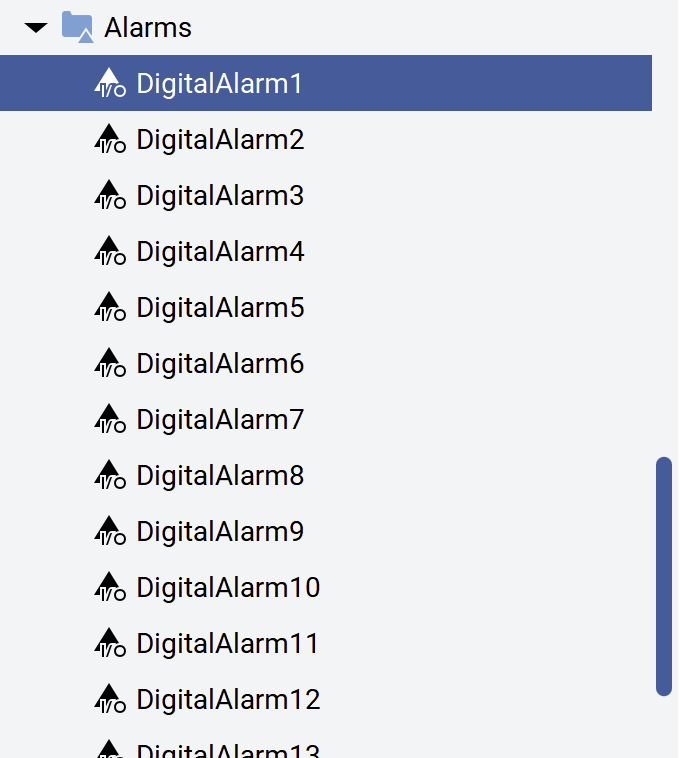
\includegraphics[width=\linewidth]{Immagini/CartellaAllarmi.png}
        \caption{Project view su \textit{Allarmi} in FT Optix™}
        \label{fig:CartellaAllarmi.png}
    \end{subfigure}
    \hfill
    % Seconda immagine
    \begin{subfigure}[t]{0.55\textwidth} % 45% della larghezza del testo
        \centering
        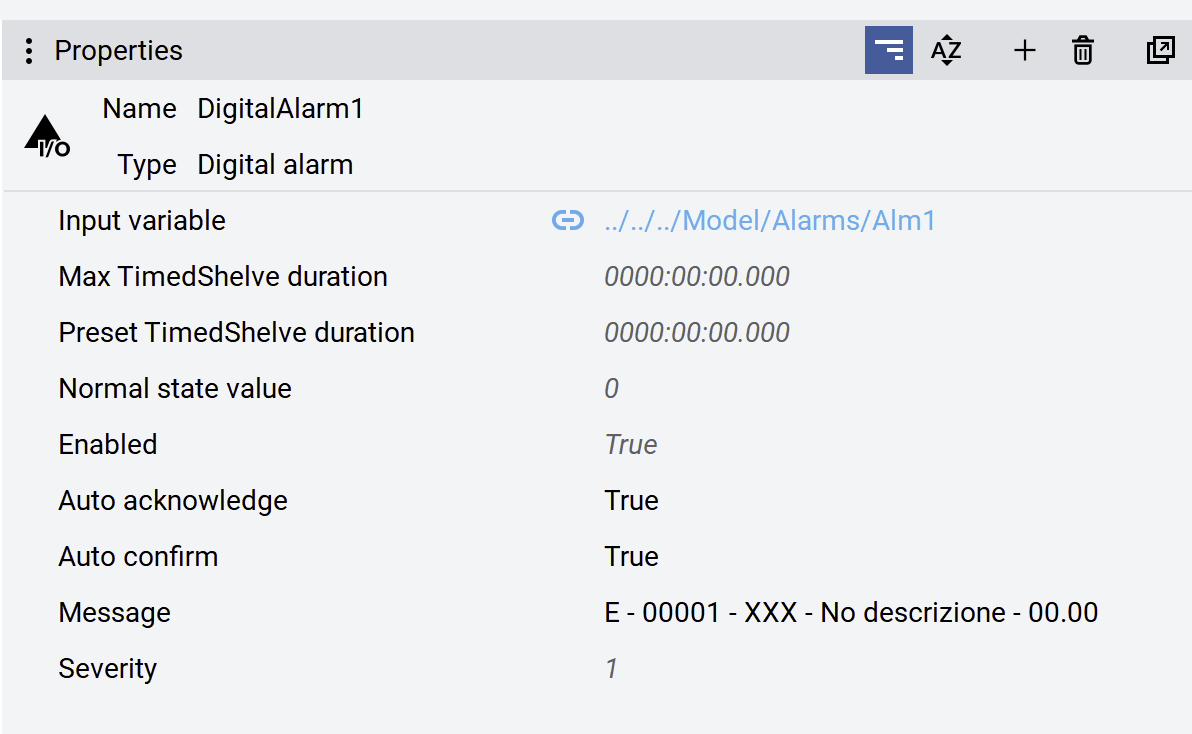
\includegraphics[width=\linewidth]{Immagini/AllarmiInfografica.png}
        \caption{Proprietà \textit{Allarmi}}
        \label{fig:AllarmiInfografica.png}
    \end{subfigure}
    \caption{Illustrazione pannelli presenti in FT Optix™}
    \label{fig:two-images00}
\end{figure}

Attraverso l'interfaccia di programma è, inoltre, possibile impostare diverse proprietà per ogni singolo allarme, come ad esempio il messaggio da visualizzare nello SCADA, la priorità e i tempi di visualizzazione del segnale (\ref{fig:AllarmiInfografica.png}). Tutta la parte di gestione degli allarmi viene poi effettuata da FT Optix™. Infine, se è necessario visualizzare i messaggi di allarme in altre sezioni, come ad esempio sul Pannello di Stato, è sufficiente richiamarli tramite funzioni specifiche di FT Optix™. In particolare, nel nostro caso, grazie alla libreria \verb|AllarmBannerlogic| il processo di visualizzazione degli allarmi viene automatizzato. Questo approccio permette di semplificare il lavoro, poiché è necessario solo inserire gli allarmi nella cartella di progetto. Naturalmente in sistemi SCADA più complessi è possibile lavorare manualmente tramite script sulla libreria, permettendo di personalizzare ulteriormente la gestione degli allarmi.

\begin{figure} [ht]
    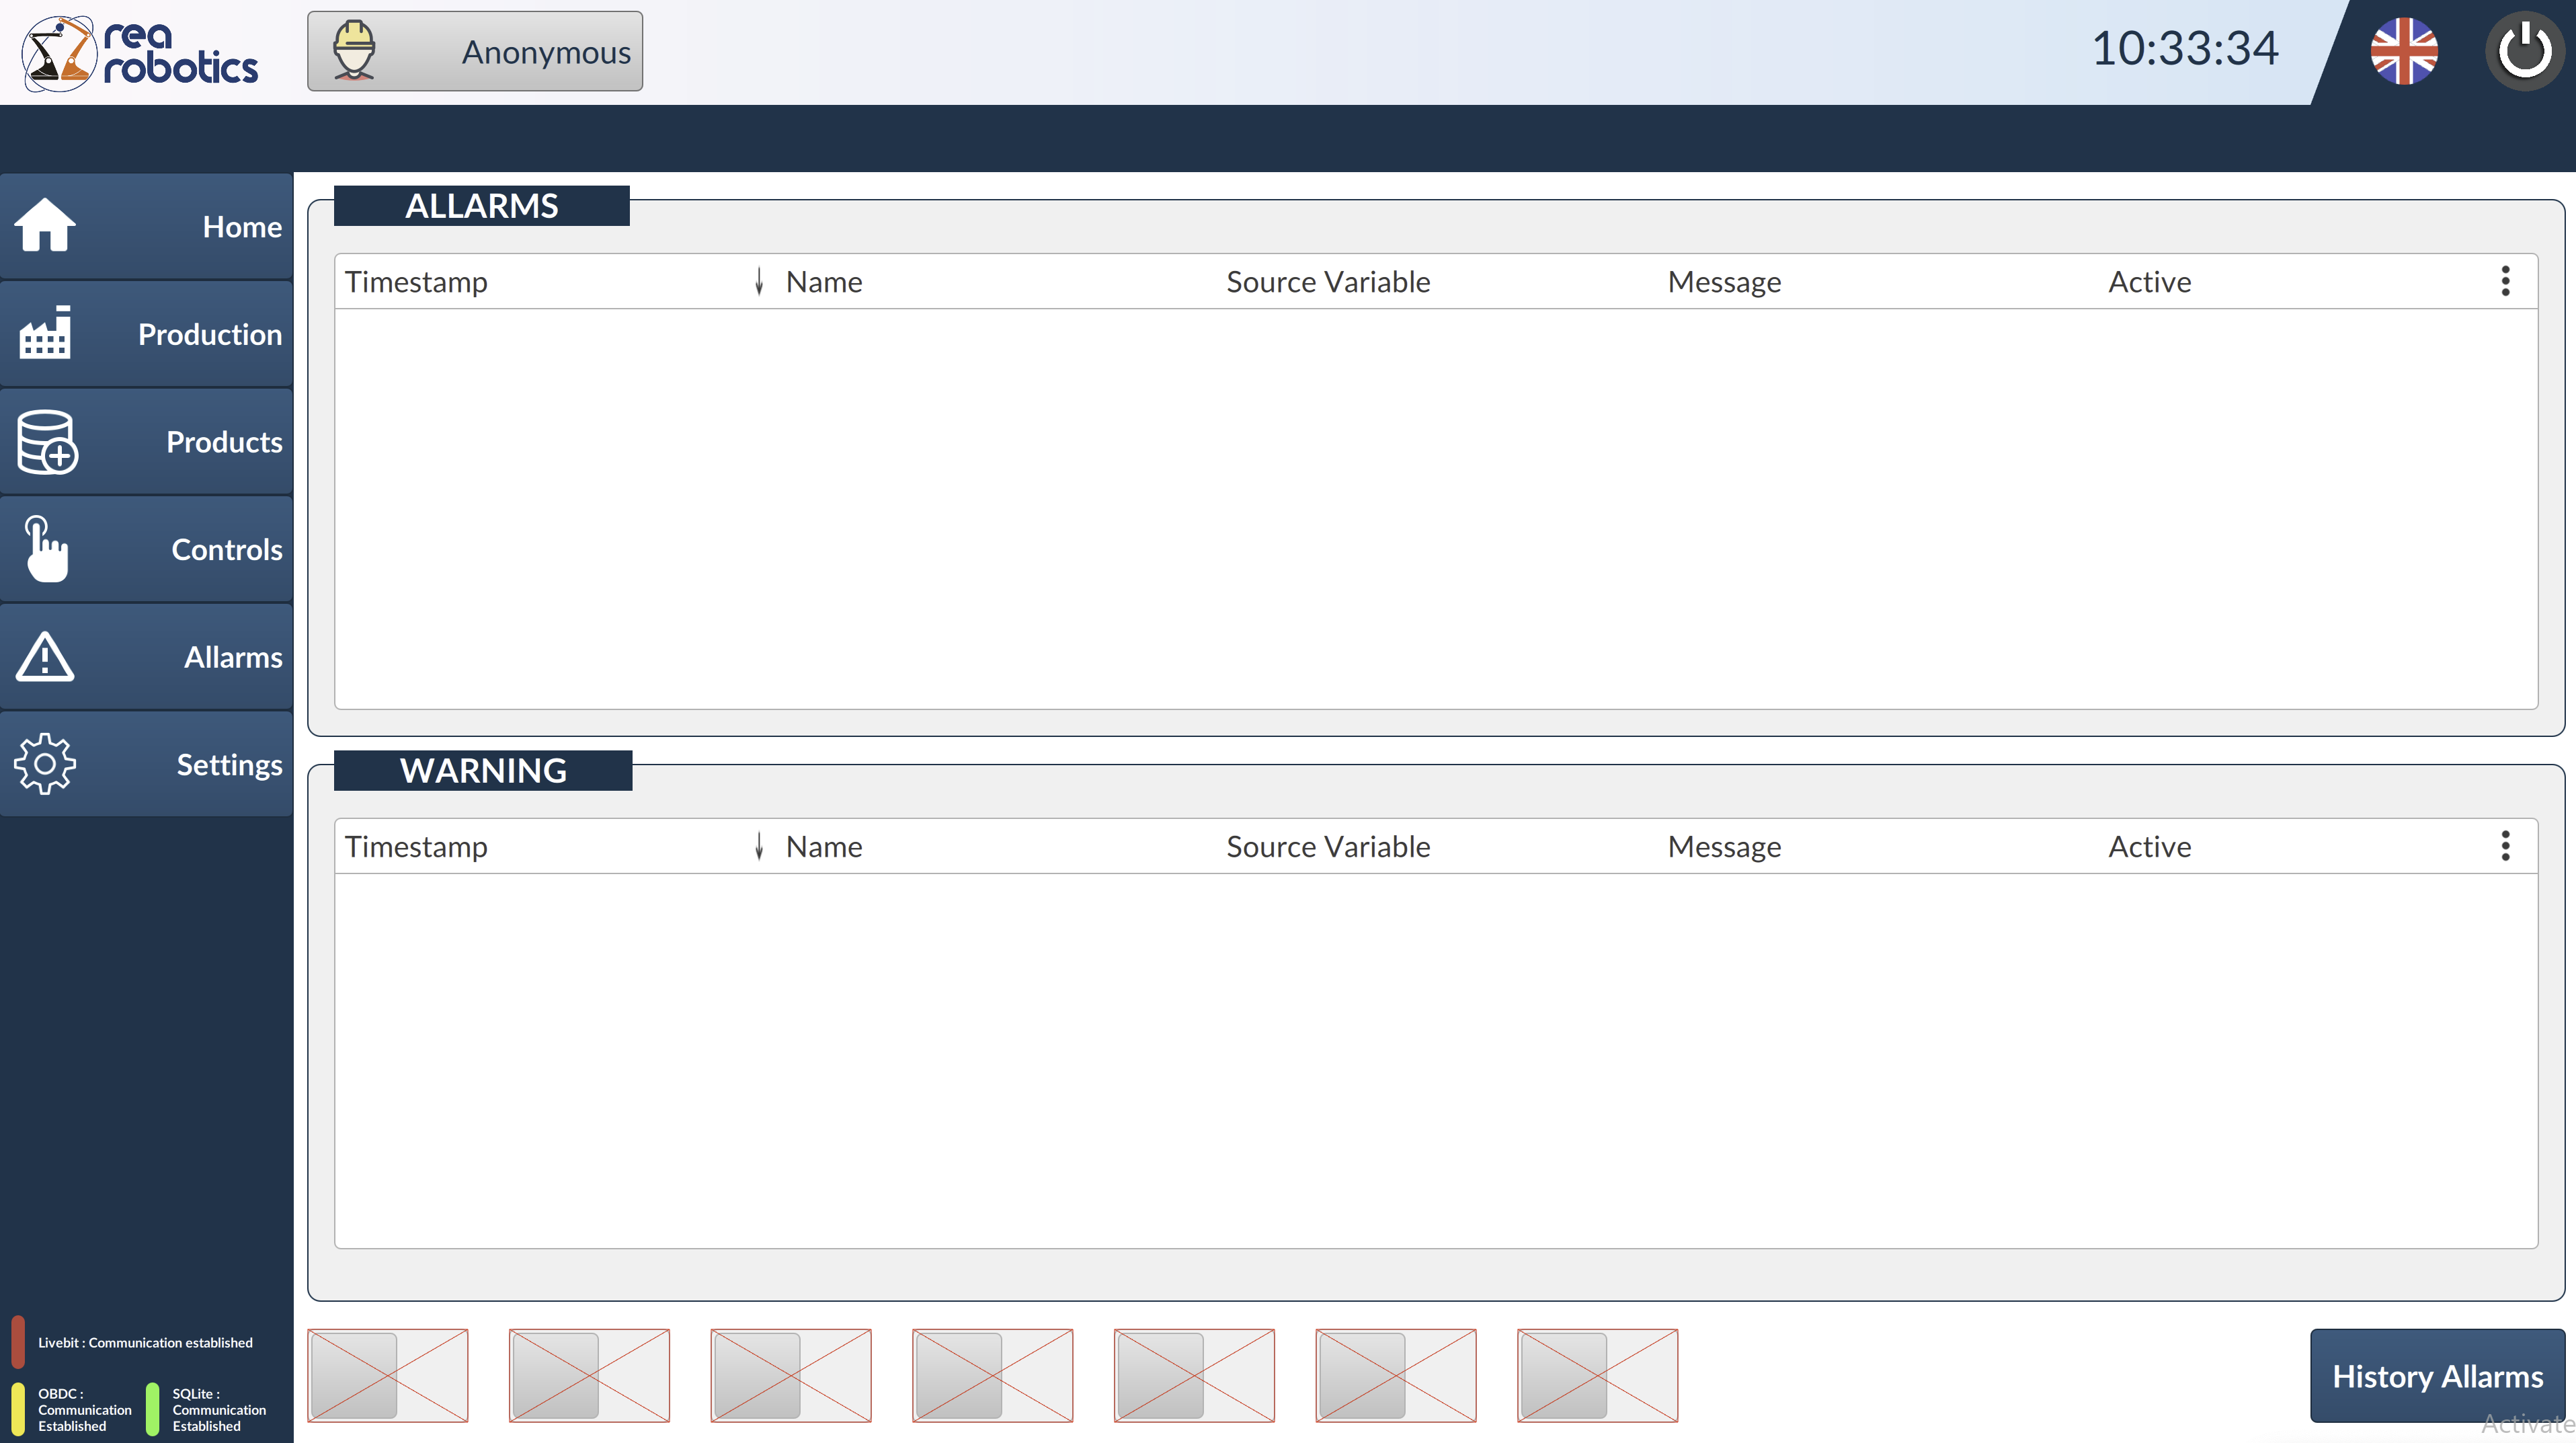
\includegraphics[width=\linewidth]{Immagini/Allarmi.png}
    \caption{Illustrazione sezione \textit{Allarmi}}
    \label{fig:Allarmi.png}
\end{figure}

\subsection{Configurazione Database aziendale}
Per quanto riguarda la parte di database aziendale, in questa sottosezione ci occuperemo della configurazione base di un database di tipo \verb|SQL Server|, come già visto per \verb|SQLite|. Inizialmente andiamo ad aggiungere all'interno della Project View, nella cartella DataStores, un oggetto di tipo \textit{ODBC database}\textsuperscript{\cite{factorytalk_odbcstore}}. A questo punto dobbiamo impostare sulle proprietà del database appena creato:
\begin{enumerate}
    \item Il DBMS type uguale a SQL Server.
    \item La struttura compresa dei vari campi delle tabelle, come già visto per \verb|SQLite|.
    \item Compilare i campi con le informazioni di accesso a SSMS
    \item Un \textit{DesignTimeNetLogic}, chiamato \verb|DesignTimeConfiguraDB| in cui andremo ad inserire informazioni fondamentali per l'utilizzo del database esterno.
\end{enumerate}
Successivamente non resta altro che replicare tutto ciò che è stato fatto per SQLite con le diverse variabili di modello, ricette e script specifici per far funzionare il database. Prima di passare al NetLogic di configurazione, è bene sottolineare che la scelta di utilizzare un database rispetto all'altro si trova all'interno della sezione Impostazioni, con la prima flag presente nel pannello. Grazie a questa flag viene cambiato il valore di una variabile booleana DB, impostando l'utilizzo delle tabelle corrette. Inoltre, questa variabile agisce sull'interfaccia di \textit{Produzione} e \textit{Articoli} visualizzata dall'operatore, che ha a disposizione due sezioni di facile utilizzo e comprensione per chi opera direttamente sul campo. Per quanto riguarda \verb|DesignTimeConfiguraDB|, è stata innanzitutto creata la classe con le costanti di riferimento del database:
\begin{csharp}
public class DesignTimeConfiguraDB : BaseNetLogic
{
    const string DB_SERVER = ".\\SQLEXPRESS";
    const string DB_NAME = "PRG_OPTIX";
    const string DB_USER = "sa";
    const string DB_PASSWORD = "reaSQL";

    private string _connectionString = $"Server={DB_SERVER};Database={DB_NAME};User Id={DB_USER};Password={DB_PASSWORD};";

    ...
\end{csharp}
Per poi configurare tramite il metodo \verb|ConfigureDB| l'accesso al database ed aggiungere eventuali tabelle necessarie al datastore OBDC di FT Optix™. Quindi, è stata copiata la libreria \verb|sni.dll| per fornire comunicazione con SQL Server, per poi aggiungere le tabelle necessarie:
\begin{csharp}
...
    sourcePath = Path.Combine(RuntimePath, "sni.dll");
    destinationPath = Path.Combine(RuntimePath, "NetSolution", "bin", "sni.dll");
    System.IO.File.Copy(sourcePath, destinationPath, true);
...
    //aggiungo le tabelle necessarie con le relative colonne
    List<string> tables = new List<string>();
    tables = ListTables();
    
    if (tables.Count>0 )
    {
        foreach (string tbl in tables)
        {
            AddNewTable(db, tbl);
        }
    }
...
\end{csharp}
Infine vengono gestiti i tipi di dati SQL, mappandoli correttamente:
\begin{csharp}
...
     static Type MapSqlType(string sqlType)
 {
     switch (sqlType.ToLower())
     {
         case "int":
             return typeof(int);
         case "varchar":
         case "nvarchar":
         case "char":
         case "nchar":
             return typeof(string);
         // Aggiungi altri casi secondo necessità
         default:
             return typeof(object); // Tipo generico per altri tipi non gestiti
     }
 }
\end{csharp}
Questo script automatizza la configurazione del collegamento ad un database SQL Server garantendo che le tabelle e le colonne siano mappate correttamente nell'ODBC dell’HMI. Nondimeno, lo script gestisce la copia delle librerie necessarie, le connessioni e soprattutto il recupero dinamico delle strutture delle tabelle, rendendo le tabelle facilmente scalabili.

\section{Sviluppo back-end e integrazione con il PLC}\label{sec:Sviluppo back-end e integrazione con il PLC}

In questa sezione analizziamo gli aspetti necessari per poter unire tutto ciò che è stato progettato finora. Lato back-end, dobbiamo garantire che lo SCADA comunichi correttamente con uno o più PLC, a seconda dell'impianto, ottenendo pieno controllo del sistema. Questo approccio permette di gestire qualsiasi caso d'uso o variabile che potrebbe comportarsi in modo imprevisto durante l'operatività della macchina. Ho deciso di focalizzare l'attenzione su due elementi chiave: la possibilità che lo SCADA determini esattamente il passo operativo del PLC in ogni momento, e la certezza che ci sia una comunicazione bidirezionale tra lo SCADA e il PLC. Per arrivare a ciò, è stata creata una macchina a stati, con un ciclo che inizia nel momento in cui la macchina viene avviata e che avanza esclusivamente in risposta ai segnali del PLC. Questa macchina rappresenta un'astrazione del comportamento del PLC, offrendo pieno controllo in qualsiasi momento. Il lavoro è stato suddiviso in più fasi:
\begin{enumerate}
    \item Inizializzazione di tutti i tag del PLC e dello SCADA.
    \item Sviluppo di un programma in grado di gestire tutti i casi d'uso e gli errori dell'impianto.
    \item Verifica che tutto sia coerente tra FT Optix™ e il Database.
\end{enumerate}

\subsection{Indicizzazione tag variabili}

L'idea a livello progettuale è stata di creare un contenitore, implementato sotto forma di classe, che raccogliesse tutti i percorsi delle variabili presenti su FT Optix™, inclusi quelli del PLC. Il primo passo consiste nell'identificare, su FT Optix™, tutte le variabili di nostro interesse. È fondamentale che sia attivata la modalità avanzata in FT Optix™ per eseguire i passi seguenti. Attraverso la \textit{Project View} vanno estrapolati i percorsi delle variabili. Ad esempio, consideriamo una variabile di modello scelta casualmente (\ref{fig:tag.png}). Una volta estratto il percorso, si ottiene una stringa di questo tipo: \verb|SCADA/Model/Produzione/ResetProduction|. Da quest'ultima conviene sempre escludere la prima parte del percorso, che rappresenta il nome del progetto, e utilizzare solo la parte rimanente. Questa scelta è motivata dal fatto che la prima parte, nel nostro caso: \verb|SCADA/| rappresenta il nome del Progetto, e se dovessimo riutilizzare tutto il modello in contesto multi-progetto, dovremmo aggiornarle globalmente tutte. Riducendo il percorso alla sola parte: \verb|Model/Produzione/ResetProduction|, si garantisce maggior flessibilità e portabilità. 

\begin{figure} [ht]
    \centering
    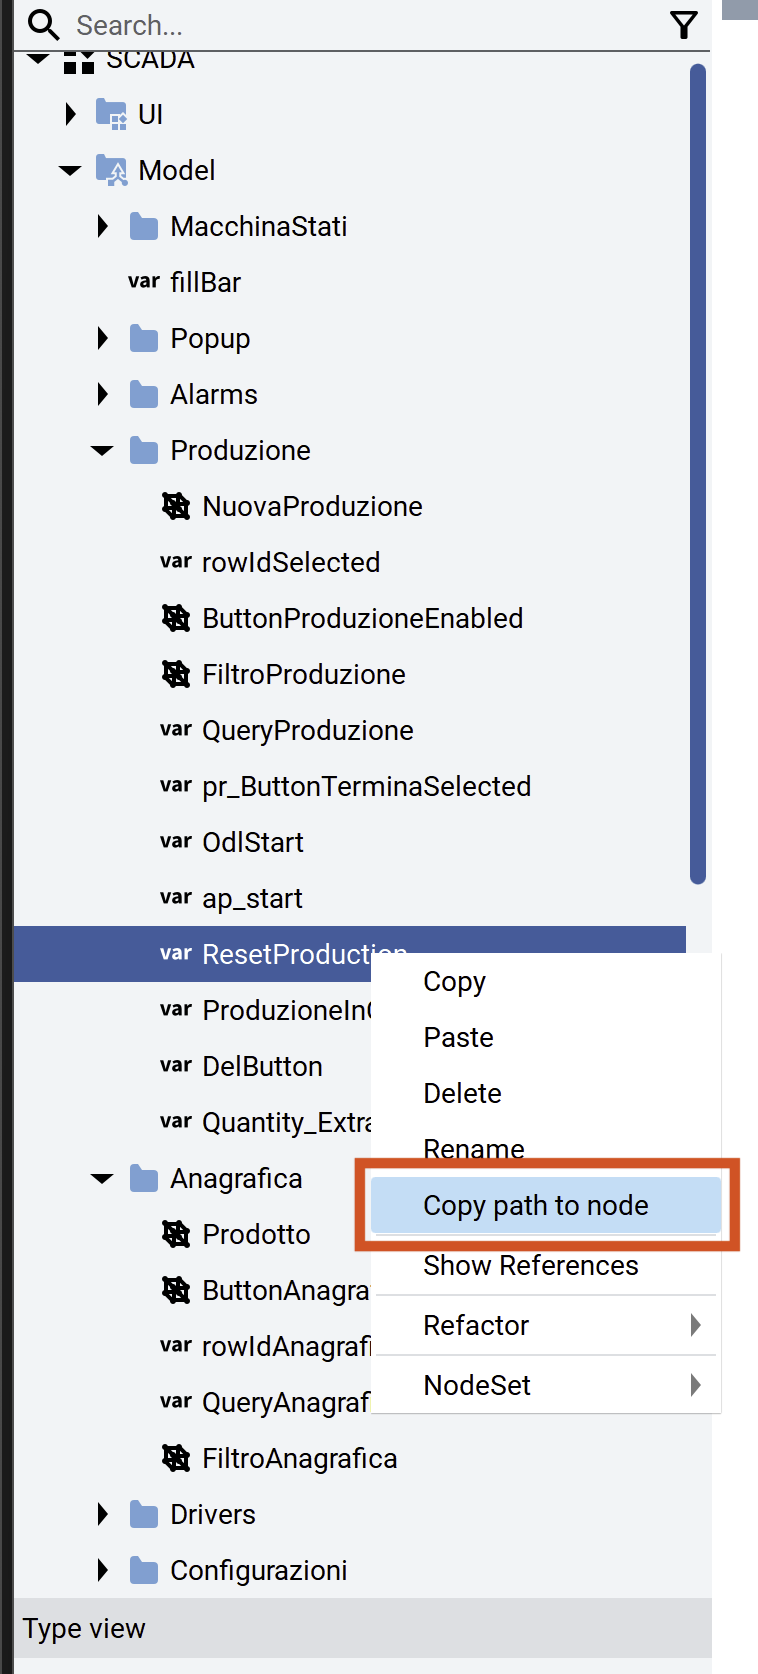
\includegraphics[width=0.3\linewidth]{Immagini/tag.png}
    \caption{esempio di salvataggio percorso variabile di modello}
    \label{fig:tag.png}
\end{figure}

Procediamo a creare la classe e ad inserire volta per volta tutti i percorsi delle variabili necessarie. Alla fine dovremmo ottenere una classe del genere:

\begin{csharp}
...

public static class VariablePaths
{
    ... // lista variabili per HMI

    //cliente_to_rea -> produzione
    public const string PathQueryProduzione                         = "Model/Produzione/QueryProduzione";
    public const string PathProduzioneFilterActive                  = "Model/Produzione/FiltroProduzione/FilterActive";
    public const string PathProduzioneTextFilter                    = "Model/Produzione/FiltroProduzione/TextFilter";
    public const string PathProduzioneAvviaEnabled                  = "Model/Produzione/ButtonProduzioneEnabled/AvviaEnabled";
    ...

    //rea_to_cliente -> storico
    public const string PathQueryStorico                            = "Model/Storico/QueryStorico";
    public const string PathStoricobdateFilter                      = "Model/Storico/bdateFilter";
    public const string PathStoricoDateFrom                         = "Model/Storico/DateFrom";
    public const string PathStoricoDateTo                           = "Model/Storico/DateTo";

    //anagrafica
    public const string PathQueryAnagrafica                         = "Model/Anagrafica/QueryAnagrafica";
    public const string PathAnagraficaFilterActive                  = "Model/Anagrafica/FiltroAnagrafica/FilterActive";
    public const string PathAnagraficaTextFilter                    = "Model/Anagrafica/FiltroAnagrafica/TextFilter";
    ...
    
    ... // lista variabili per HMI
\end{csharp}

Nella classe sono state inserite variabili secondo una precisa struttura: il percorso salvato in precedenza associato ad una stringa. Questo approccio consente maggiore controllo delle variabili all'interno della macchina a stati e, qualora sia necessario, permette di aggiungere nuove variabili semplicemente aggiornando la suddetta classe. È inoltre consigliato, ma non estremamente essenziale, suddividere le variabili secondo una logica ben definita in modo che siano facilmente rintracciabili, specialmente in impianti enormemente più strutturati.

Per la gestione delle variabili nella macchina a stati è stata definita una regola di suddivisione in due tipologie principali per fornire maggiore sicurezza:
\begin{enumerate}
    \item \textbf{DB92-PLCtoHMI}: sono tutte le variabili gestite dal controllore logico programmabile e inviate all'HMI, che le può leggere ma non modificare.
    \item \textbf{DB91-HMItoPLC}: variabili gestite sempre dal PLC, ma scrivibili solo dallo scada e leggibili dal PLC.
\end{enumerate}
Questa classificazione rimane costante indipendentemente dall'impianto; ciò che cambierà sono la quantità e il tipo di segnale dei tag. Nel caso specifico, verranno considerate le variabili utilizzate in un impianto di piegatura, che sarà analizzato più dettagliatamente nel capitolo \ref{sec:CasoStudio}. 

\subsection{Sviluppo Macchina a Stati}

 Dal lato progettazione, è stato inserito un oggetto \textit{RunTimeNetLogic} associato alla \textit{MainWindow}. Per quanto concerne la programmazione, lo script associato è stato suddiviso in diverse parti. Inizialmente, vengono dichiarati alcuni script strettamente legati al database, che vengono richiamati all'interno della \verb|StateMachine|. Successivamente, all'interno della funzione \verb|Start| (riga 19), è stata definita una \verb|PeriodicTask| con i seguenti attributi: 
 \begin{itemize}
     \item \verb|Maincycle|: contiene la logica periodica del sistema
     \item \verb|250ms|: indica la frequenza con cui la logica viene ripetuta periodicamente 
     \item \verb|LogicObject|: contiene le risorse necessarie per l'esecuzione.
 \end{itemize}
Grazie a questa configurazione, dopo aver avviato l'impianto, il maincycle viene eseguito ogni 250ms. Questa frequenza garantisce una sincronizzazione quasi istantanea tra HMI e PLC, riducendo al minimo gli errori.

\begin{csharp}
...
public class script_maincycle : BaseNetLogic
{
    private PeriodicTask myPeriodicTask;
    private RuntimeNetLogicClienteToRea _prod;
    private RuntimeNetLogicAnagrafica _art;

    private RuntimeNetLogicClienteToReaLocale _prodLocale;
    private RuntimeNetLogicAnagraficaLocale _artLocale;

    public override void Start()
    {
        _prod = new RuntimeNetLogicClienteToRea();
        _art = new RuntimeNetLogicAnagrafica();

        _prodLocale = new RuntimeNetLogicClienteToReaLocale();
        _artLocale = new RuntimeNetLogicAnagraficaLocale();

        myPeriodicTask = new PeriodicTask(Maincycle, 250, LogicObject);
        myPeriodicTask.Start();

    }

    public override void Stop()
    {
        myPeriodicTask.Dispose();
    }

    public void Maincycle()
    {
        StateMachine();
    }

    private void StateMachine()
    {
    ...
\end{csharp}

La struttura della\verb|StateMachine| è stata organizzata in diverse sezioni. La prima si occupa di inizializzare le variabili, richiamando i percorsi definiti nella classe \verb|VariablePaths| illustrata in precedenza, che contiene tutti i tag di interesse. Di seguito, una parte del codice illustrato:

\begin{csharp}
...
    private void StateMachine()
{
    //inizializzo variabili plc
    PopUpNetLogic popup                             = new PopUpNetLogic();
    var popupOK                                     = Project.Current.GetVariable(VariablePaths.PathPopupOK);
    var popupYes                                    = Project.Current.GetVariable(VariablePaths.PathPopupYes);
    var popupNo                                     = Project.Current.GetVariable(VariablePaths.PathPopupNo);

    var MachineStatusText                           = Project.Current.GetVariable(VariablePaths.PathMachineStatusText);
    var MachineStatus                               = Project.Current.GetVariable(VariablePaths.PathMachineStatus);
    var OdlStart                                    = Project.Current.GetVariable(VariablePaths.PathOdlStart);
    long OdlStartLong                               = OdlStart.Value; 
    var ap_start                                    = Project.Current.GetVariable(VariablePaths.Pathap_start);
    var pr_ButtonTerminaSelected                    = Project.Current.GetVariable(VariablePaths.Pathpr_ButtonTerminaSelected);
    var ResetProduction                             = Project.Current.GetVariable(VariablePaths.PathResetProduction);
    var ProduzioneInCorso                           = Project.Current.GetVariable(VariablePaths.PathProduzioneInCorso);

    var DB91_CambioProduzione                       = Project.Current.GetVariable(VariablePaths.PathDB91_CambioProduzione);
    var DB91_TerminaProduzione                      = Project.Current.GetVariable(VariablePaths.PathDB91_TerminaProduzione);
    ... // altre variabili plc
\end{csharp}
Dopo l'indicizzazione, la macchina stati è composta da vari passi definiti all'interno di uno \verb|switch-case| e numerati da 0 a 199, ciascuno per uno specifico stato operativo. Questo approccio logico è ampiamente utilizzato negli impianti industriali in REA, in quanto consente di gestire in modo modulare e scalabile le varie operazioni dallo scada oltre a facilitare la manutenzione futura. Di seguito, una panoramica dei passi standard:
\begin{itemize}
    \item \verb|0 = "Inizializzazione"|: passo che identifica l'avvio della macchina, solitamente corrisponde alla schermata di caricamento dell'HMI.
    \item \verb|1 = "Stato iniziale (IDLE)"|: passo in cui avviene un reset completo delle variabili HMI e DB91.
    \item \verb|10 = "Controllo allineamento con PLC-SCADA"|: sincronizzazione tra SCADA e PLC.
    \item \verb|20 = "Attesa avvio produzione"|: stato di attesa, con macchina operativa per la produzione.
    \item \verb|70 = "Attesa esito da PLC - ok/ko"|: attesa del segnale di risposta dal PLC dopo un comando inviato dall'HMI.
    \item \verb|80 = "Attesa RESET segnali da PLC - ok/ko"|: verifica di sicurezza, attesa ulteriore segnale dal PLC.
    \item \verb|100 = "IN LAVORO"|: identifica che l'impianto è in piena attività produttiva.
    \item \verb|150 = "Fine produzione + attesa handshake PLC"|: stato di attesa del segnale di handshake da parte del PLC.
    \item \verb|165 = "Attesa reset richiesta termina produzione dal PLC"|: pulizia delle variabili per garantire la sicurezza operativa.
    \item \verb|190 = "ANNULLAMENTO CARICAMENTO DA OPERATORE"| annullamento di qualsiasi produzione attiva o in chiusura.
    \item \verb|199 = "Termina produzione completata correttamente"| controllo finale e ritorno al passo 20.
\end{itemize}
Come si può notare, non tutti i passi seguono un ordine sequenziale; questo consente di aggiungere eventuali estensioni future agli impianti. Partiamo con l'analizzare il codice di tutti i passi principali, escludendo l'implementazione di alcuni per l'impianto di piegatura, che analizzeremo successivamente nel capitolo \ref{sec:CasoStudio}.

Il codice di \verb|case 0| rappresenta la prima iterazione del ciclo e quindi l'avvio della macchina. Qui si gestisce il caricamento iniziale, inclusa l'interfaccia HMI. Viene monitorata la variabile \verb|fillBar|, cioè la barra di caricamento, per verificare che l'intero programma sia caricato (righe 7-10). Una volta completato il caricamento, lo stato viene impostato a 1, e nell'HMI viene caricata la pagina iniziale completa di tutta l'interfaccia (righe 13-20). Infine esce dal passo.
\begin{csharp}
...
    case 0:
        //-------------------------------------------
        MachineStatusText.Value = "Inizializzazione";
        //-------------------------------------------
    
        if (Project.Current.GetVariable("Model/fillBar").Value <15)
        {
            Project.Current.GetVariable("Model/fillBar").Value += 1;
        }
        else
        {
            MachineStatus.Value = 1;
            
            //cambia pagina
            var myPanel = LogicObject.GetPanelLoader("PanelLoader1");
            myPanel.ChangePanel("Main");
    
            var mainPanel = LogicObject.GetPanelLoader("PanelLoaderScreens");
            mainPanel.ChangePanel("Home");
        }
    
        break;
...
\end{csharp}
Il \verb|case 1| rappresenta uno dei passi più critici, poiché si occupa di controllare variabili, allarmi e sensori sia dell'HMI che del PLC. Questo passo è importante per garantire continuità in caso di blackout o spegnimenti anomali del pannello HMI, che potrebbero de sincronizzare PLC-SCADA. Al suo interno vengono eseguiti i seguenti reset:
\begin{enumerate}
    \item \verb|DB91_CambioProduzione.Value|: impostato a false (riga 7).
    \item \verb|ResetHMIProductVar()|: richiama la funzione di reset delle variabili HMI di produzione (riga 10).
    \item \verb|ResetPLCProductVar()|: richiama la funzione di reset delle variabili PLC (riga 13).
\end{enumerate}
Concluso il reset, la macchina imposta il passo successivo, cioè 10, ed esce dal passo (riga 15).
\begin{csharp}
...
    case 1:   
        //------------------------------------------------
        MachineStatusText.Value = "Stato iniziale (IDLE)";
        //------------------------------------------------
    
        DB91_CambioProduzione.Value = false;
    
        //Reset di tutte le variabili legate al caricamento programma su HMI
        ResetHMIProductVar();
    
        //Reset variabili PLC DB91
        ResetPLCProductVar();
    
        MachineStatus.Value = 10;
    
        break;
...
\end{csharp}
Dal \verb|case 10| tutto il codice è stato strutturato con l'implementazione sia per il database locale, sia per il database aziendale. Tuttavia, in questa spiegazione ci concentriamo su una singola implementazione, poiché le logiche principali rimangono identiche. Per prima cosa avviene un check sulla variabile \verb|DBExpress.Value| configurata nelle impostazioni dell'HMI che determina quale database è in utilizzo (riga 7). Fatto questo avviene un confronto diretto con la variabile di status nel PLC (riga 17): se maggiore di 0, il PLC sta già lavorando ad un ordine. In questo caso, tutte le variabili dello SCADA vengono aggiornate per riallinearsi con il PLC e continuare la produzione senza problemi (righe 20-29); se invece \verb|DB92_ODP.Value| è uguale a zero, il sistema procede al passo successivo senza ulteriori azioni (riga 33). 
\begin{csharp}
...
    case 10:
    //---------------------------------------------------------------
    MachineStatusText.Value = "Controllo allineamento con PLC-SCADA";
    //---------------------------------------------------------------

    if (DBExpress.Value)
    {
       ... //implementazione per SSMS
    }
    else
    {
        //sincronizzo il campo /Status con lo stato corretto dell'ordine che sta girando sul PLC
        _prodLocale.pr_StatusSyncro_Locale(DB92_ODP.Value);

        //se in plc sto lavorando con una ricetta allineo tabella in running
        if (DB92_ODP.Value > 0)
        {
            //Sincronizzo OdlStart
            OdlStartLong = DB92_ODP.Value;

            //mando prodotti al plc
            SendProductDataToPLCLocale(OdlStartLong);

            //mi metto in produzione in corso 
            ProduzioneInCorso.Value = true;

            //vado in produzione
            MachineStatus.Value = 100;
        }
        else
        {
            MachineStatus.Value = 20;
        }
    }

    break;
...
\end{csharp}
Il \verb|case 20| rappresenta lo stato in cui l'impianto è in attesa avvio produzione, monitorando continuamente le seguenti variabili (riga 12): 
\begin{itemize}
    \item \verb|ap_start.Value|: è stato avviato un ordine dall'operatore.
    \item \verb|OdlStartLong|: è maggiore di zero se esiste un ordine di produzione in attesa.
\end{itemize}
Se avvengono queste condizioni, i dati relativi all'ordine vengono inviati al PLC tramite funzione \verb|SendProductDataToPLCLocale| (riga 15). Se avviene l'invio, viene impostata \verb|ProduzioneInCorso.Value| a TRUE (riga 18), con  cambio al passo successivo (riga 21). In caso contrario viene aperto un popup di avvertimento e conseguentemente cambiato il passo (righe 26, 27).
\begin{csharp}
...
    case 20:
    //--------------------------------------------------
    MachineStatusText.Value = "Attesa avvio produzione";
    //--------------------------------------------------
    if (DBExpress.Value)
    {
        ... //implementazione per SSMS
    }
    else
    {
        if (ap_start.Value && OdlStartLong > 0)
        {
            //mando dati al plc
            if (SendProductDataToPLCLocale(OdlStartLong))
            {
                //vado in produzione in corso
                ProduzioneInCorso.Value = true;

                //cambio stato
                MachineStatus.Value = 25;
            }
            else
            {
                //Dati anagrafica non esistenti, popup e KO diretto
                popup.OpenPopUp("Dati anagrafica non esistenti: crea prima l'articolo in Anagrafica", 0);
                MachineStatus.Value = 21;
            }
        }
    }
    
    break;
...
\end{csharp}
Il \verb|case 21| gestisce l'attesa di lettura del popup da parte dell'operatore, procedendo al ripristino delle variabili di produzione e al cambio del passo. Nel \verb|case 25| viene impostata la variabile di cambio produzione a TRUE (riga 13), per avvisare il PLC del cambio di ordine. Viene aggiornato l'attributo dello stato dell'ordine nel database (riga 16), e viene richiamata la funzione per abilitare/disabilitare i pulsanti della schermata di produzione. Infine cambiamo passo (riga 19).
\begin{csharp}
...
    case 25:
    //---------------------------------------------------------
    MachineStatusText.Value = "Invio cambio produzione al PLC";
    //---------------------------------------------------------
    if (DBExpress.Value)
    {
        ... //implementazione per SSMS
    }
    else
    {
        //Handshake PLC - attendo risposta
        DB91_CambioProduzione.Value = true;

        //Aggiorno stato in db
        _prodLocale.pr_UpdateStatusLocale(OdlStartLong, MachineStatus.Value);

        //Aggiorno pulsanti
        _prodLocale.pr_ManageProductionButtonsLocale(MachineStatus.Value);

        //Cambio stato
        MachineStatus.Value = 50;
    }

    break;
...
\end{csharp}
I passi \verb|case 50, 55, 60| verranno trattati nel Capitolo \ref{sec:CasoStudio}, essendo progettati secondo l'impianto su cui gira lo SCADA. Se tutto risulta corretto arriviamo al \verb|case 70| in cui siamo in attesa dell'esito da parte del PLC relativo al cambio produzione:
\begin{enumerate}
    \item Il PLC da l'OK (da riga 8): allora vengono resettate le variabili precedenti di cambio produzione e caricamento ordine, per poi cambiare passo.
    \item Il PLC mi manda un KO (da riga 21): allora l'HMI mostra a schermo l'errore e rimane in attesa di risposta da parte dell'operatore.
\end{enumerate}
\begin{csharp}
...
    case 70:
    //------------------------------------------------------
    MachineStatusText.Value = "Attesa esito da PLC - ok/ko";
    //------------------------------------------------------

    //Se ricevo OK
    if (DB92_CambioProduzioneOK.Value)
    {
        //reset bit di cambio produzione
        DB91_CambioProduzione.Value = false;

        //reset richiesta caricamento nuovo prodotto
        ap_start.Value = false;

        //cambio stato
        MachineStatus.Value = 80;
    }

    //Se ricevo KO
    if (DB92_CambioProduzioneKO.Value)
    {
        //mostra popup
        popup.OpenPopUp("KO da PLC: dati errati", 0);

        //Cambio stato
        MachineStatus.Value = 71;
    }

    break;
...
\end{csharp}
Il \verb|case 71| gestisce il reset della variabile del popup mostrato in errore e passa direttamente al 180 (ne discuteremo l'implementazione in seguito). Il \verb|case 80| attende che il PLC resetti entrambi i segnali precedenti (riga 12), successivamente cambia il passo per avviare la produzione (riga 15), e aggiorna nuovamente lo stato dell'ordine nel database (riga 18) e i pulsanti dell'HMI (riga 21).
\begin{csharp}
...
    case 80:
    //--------------------------------------------------------------
    MachineStatusText.Value = "Attesa RESET segnali da PLC - ok/ko";
    //--------------------------------------------------------------
    if (DBExpress.Value)
    {
        ... //implementazione per SSMS
    }
    else
    {
        if (!DB92_CambioProduzioneOK.Value && !DB92_CambioProduzioneKO.Value)
        {
            //Cambio stato
            MachineStatus.Value = 100;

            //Aggiorno status in db
            _prodLocale.pr_UpdateStatusLocale(OdlStartLong, MachineStatus.Value);

            //Aggiorno pulsanti
            _prodLocale.pr_ManageProductionButtonsLocale(MachineStatus.Value);
        }
    }
    
    break;
...
\end{csharp}
Il \verb|case 100| rappresenta il cuore del processo produttivo, in cui la macchina lavora sull'ordine e aggiorna continuamente i dati relativi alla produzione. Per prima cosa viene selezionato il database con annessi campi per l'aggiornamento dei dati durante la produzione. Successivamente vengono mandate continuamente richieste al PLC in cui viene controllato che i pezziDepositati, quindi i pezzi prodotti, siano uguali a quelli memorizzati dall'HMI. In caso di discrepanza, si aggiorna il database e si sincronizzano i valori in memoria (righe 10-14). Questo avviene finché non si raggiunge la quantità richiesta, sommata all'extra produzione (riga 18), che inizialmente sarà a 0. Di seguito se l'operatore preme il pulsante di fine produzione, resetta il flag e cambia stato a fine produzione (righe 21-24). Nel codice sottostante vengono illustrate anche alcune parti fondamentali delle funzioni ausiliarie di aggiornamento parametri richiamate precedentemente.
\begin{csharp}
...
    case 100:
    //------------------------------------
    MachineStatusText.Value = "IN LAVORO";
    //------------------------------------
    // Seleziona il data store e i nomi dei campi in base a DBExpress.Value
    ...

    // Aggiorna le quantità se necessario
    if (DB92_PezziDepositati.Value != Mem_PezziDepositati.Value ||
        DB92_PezziScarti.Value != Mem_PezziScarti.Value ||
        DB92_QtaRiordino.Value != Mem_QtaRiordino.Value)
    {
        AggiornaQuantita(myStore, tableName, idField, quantityProducedField, totalRejectField);
    }

    // Verifica se è stata raggiunta la quantità richiesta più l'extra produzione
    ControllaExtraProduzione(myStore, tableName, idField, quantityRequestedField, extraProductionField);

    // Gestisce la richiesta di fine produzione
    if (pr_ButtonTerminaSelected.Value)
    {
        pr_ButtonTerminaSelected.Value = false;
        MachineStatus.Value = 148; // Codice di stato per "fine produzione"
    }

    // Funzione per aggiornare le quantità
    void AggiornaQuantita(... //variabili richieste)
    {
        ...
        // Aggiorna quantità pezzi prodotti
        if (DB92_PezziDepositati.Value != Mem_PezziDepositati.Value)
        {
            string query = $"UPDATE {table} SET {quantityProducedFieldName} = '{(uint)DB92_PezziDepositati.Value}' WHERE {idFieldName} = '{OdlStartLong}'";
            store.Query(query, out Header, out ResultSet);
            Mem_PezziDepositati.Value = DB92_PezziDepositati.Value;
        }

        // Aggiorna quantità scarti
        if (DB92_PezziScarti.Value != Mem_PezziScarti.Value)
        {
            string query = $"UPDATE {table} SET {totalRejectFieldName} = '{(uint)DB92_PezziScarti.Value}' WHERE {idFieldName} = '{OdlStartLong}'";
            store.Query(query, out Header, out ResultSet);
            Mem_PezziScarti.Value = DB92_PezziScarti.Value;
        }

        // Aggiorna quantità di riordino
        if (DB92_QtaRiordino.Value != Mem_QtaRiordino.Value)
        {
            string query = $"UPDATE {table} SET {quantityProducedFieldName} = '{(uint)DB92_PezziDepositati.Value}' WHERE {idFieldName} = '{OdlStartLong}'";
            store.Query(query, out Header, out ResultSet);
            Mem_QtaRiordino.Value = DB92_QtaRiordino.Value;
        }
    }

    // Funzione per controllare l'extra produzione
    void ControllaExtraProduzione(... //variabili richieste)
    {
        ...
        string query = $"SELECT {quantityRequestedFieldName}, {extraProductionFieldName} FROM {table} WHERE {idFieldName} = '{OdlStartLong}'";
        store.Query(query, out HeaderExtra, out ResultSetExtra);

        int quantityRequested = Convert.ToInt32(ResultSetExtra[0, 0]);
        int extraProduction = Convert.ToInt32(ResultSetExtra[0, 1]);

        // Richiesta per extra-produzione
        if (DB92_PezziDepositati.Value >= quantityRequested + extraProduction)
        {
            MachineStatus.Value = 110; // Codice di stato per "extra produzione raggiunta"
        }
    }
    break;
...
\end{csharp}
Illustriamo anche la gestione di extra produzione tramite popup, eseguita tramite il codice seguente. Il tutto è strutturato su due \verb|case|, il \verb|110| che gestisce l'apertura del popup e il \verb|111| che gestisce le risposte attese dal popup. Nello specifico deve gestire sia la terminazione della produzione senza aggiunta di extra (righe 10-14), sia, in caso affermativo, il ritorno allo stato di produzione (da riga 18).
\begin{csharp}
...
    case 111:
    //---------------------------------------------
    MachineStatusText.Value = "Attesa di conferma";
    //---------------------------------------------
    // Seleziona il data store e i nomi dei campi in base a DBExpress.Value
    ...

    // Richiesta fine produzione
    if (pr_ButtonTerminaSelected.Value)
    {
        pr_ButtonTerminaSelected.Value = false;
        DB91_TerminaProduzione.Value = true;
        MachineStatus.Value = 150;
    }

    // Ritorno in produzione
    if (Extra_Produzione.Value)
    {
        Extra_Produzione.Value = false;
        DB91_RiordinoProduzione.Value = true;

        // Recupera il valore di Extra_Production
        Object[,] ResultSetOldExtra;
        String[] HeaderOldExtra;
        string queryOldE = $"SELECT {extraProductionFieldPopup} FROM {tableNamePopup} WHERE {idFieldPopup} = '{OdlStartLong}'";
        myStoreE.Query(queryOldE, out HeaderOldExtra, out ResultSetOldExtra);
        int OldExtraProduction = Convert.ToInt32(ResultSetOldExtra[0, 0]);

        // Aggiorna Quantity_ExtraProduzione
        Quantity_ExtraProduzione.Value += OldExtraProduction;

        // Aggiorna il database
        Object[,] ResultSet;
        String[] Header;
        string query = $"UPDATE {tableNamePopup} SET {extraProductionFieldPopup} = '{(uint)Quantity_ExtraProduzione.Value}' WHERE {idFieldPopup} = '{OdlStartLong}'";
        myStoreE.Query(query, out Header, out ResultSet);

        // Cambio stato
        MachineStatus.Value = 100;
    }
    break;
...
\end{csharp}
Se il processo produttivo è avvenuto correttamente, ci troveremo al \verb|case 148| in cui viene richiesto all'operatore di confermare la chiusura ordine. Le varie risposte sono gestite al \verb|case 149|, in cui vengono gestiti i comandi di reset popup, il \verb|DB91_TerminaProduzione| è il prossimo passo a cui passare. Nel caso in cui venga confermata la chiusura ordine, lo scopo del \verb|case 150| è di rimanere in attesa dell'handshake da parte del PLC, cioè la variabile \verb|DB92_AckTerminaProduzione|. Se tutto avviene in modo corretto, vengono resettate tutte le variabili di produzione (righe 10-14) e si passa al \verb|case 160| in cui viene fatto l'aggiornamento delle tabelle spostando la produzione appena conclusa in storico produzione. Il \verb|case 165| monitora il reset della variabile \verb|DB92_AckTerminaProduzione| di handshake e imposta il passo direttamente a quello finale. 
\begin{csharp}
...
    case 150:
    //-----------------------------------------------------------------
    MachineStatusText.Value = "Fine produzione + attesa handshake PLC";
    //-----------------------------------------------------------------

    //rimango in attesa dell'ack PLC
    if (DB92_AckTerminaProduzione.Value)
    {
        DB91_TerminaProduzione.Value = false;

        ProduzioneInCorso.Value = false;

        MachineStatus.Value = 160;
    }

    break;

    case 160:
    //----------------------------------------------------------------------------
    MachineStatusText.Value = "Aggiornamento tabelle e spostamento nello storico";
    //----------------------------------------------------------------------------
    if (DBExpress.Value) {
        ... //implementazione per SSMS
    }
    else
    {
        //Aggiorno stato in db
        _prodLocale.pr_UpdateStatusLocale(OdlStartLong, MachineStatus.Value);

        //Aggiorno pulsanti
        _prodLocale.pr_ManageProductionButtonsLocale(MachineStatus.Value);

        //sposto su storico e elimino record
        _prodLocale.pr_TerminateAllRunningLocale();
        _prodLocale.pr_EliminaLocale(OdlStart.Value);

        //reset variabili
        ResetHMIProductVar();
        ResetPLCProductVar();

        MachineStatus.Value = 165;
    }
    
    break;
...
\end{csharp}
I passi \verb|case 180, 181, 190 e 191| servono per gestire i vari KO in cui ci siamo imbattuti durante tutto il processo e che sono stati rispettivamente richiamati.
\begin{itemize}
    \item \verb|case 180 = errore caricamento ricetta KO da PLC|: segnala un qualsiasi errore nel caricamento della ricetta da parte del PLC, aggiornando lo stato nel database e resettando le variabili sia del PLC, sia dell'HMI, per poi passare al passo successivo.
    \item \verb|case 181 = Attesa rimozione segnali KO da PLC|: il sistema è in attesa che i segnali di KO vengano rimossi dal PLC, passando poi al passo 199.
    \item \verb|case 190 = annullamento caricamento da operatore|: gestisce l'annullamento manuale del caricamento della ricetta da parte dell'operatore, aggiornando stato, pulsanti e resettando variabili. Di seguito viene riportata una parte del codice.
    \item \verb|case 191 = Attesa fine produzione da PLC|: il sistema attende una conferma di terminazione di produzione da parte del PLC, passando poi al passo finale.
\end{itemize}
\begin{csharp}
...
    case 190:
    //----------------------------------------------------------------
    MachineStatusText.Value = "ANNULLAMENTO CARICAMENTO DA OPERATORE";
    //----------------------------------------------------------------
    if (DBExpress.Value)
    {
        ... //implementazione per SSMS
    }
    else
    {
        //aggiorno status
        _prodLocale.pr_UpdateStatusLocale(OdlStartLong, MachineStatus.Value);

        //aggiorno pulsanti
        _prodLocale.pr_ManageProductionButtonsLocale(MachineStatus.Value);

        ResetHMIProductVar();
        ResetPLCProductVar();

        DB91_TerminaProduzione.Value = true;

        MachineStatus.Value = 191;
    }

    break;
...
\end{csharp}
Infine, il \verb|case 199| finalizza il processo e riporta la macchina in attesa di un nuovo ciclo produttivo, quindi in attesa di avvio produzione \verb|case 20|. Questo passo vale sia in caso di avvenuta produzione precedente, sia nel caso in cui non sia stato prodotto nulla per errori di percorso.
\begin{csharp}
...
        case 199:
        //----------------------------------------------------------------------
        MachineStatusText.Value = "Termina produzione completata correttamente";
        //----------------------------------------------------------------------

        if (!DB92_AckTerminaProduzione.Value)
        {
            MachineStatus.Value = 20;
        }

        break;

    default:
        break;
}
...
\end{csharp}
In questo capitolo abbiamo analizzato i punti salienti del main cycle. Per visionare il codice completo far riferimento alla repository GitHub, più precisamente al file: \verb|script_maincycle.cs|.

